% \documentclass[nohyper,nobib]{tufte-book}
\documentclass[a4paper,nohyper,nobib,openany,justified]{tufte-book}
\usepackage{nameref}
% \hypersetup{colorlinks,urlcolor=blue,linkcolor=blue}% uncomment this line if you prefer colored hyperlinks (e.g., for onscreen viewing)
% \usepackage{natbib}
% \setcitestyle{authoryear}
\usepackage{url}
\usepackage{multirow}
\usepackage{amsmath}
\usepackage{amssymb}
\usepackage{scrextend}
\usepackage{setspace}
\changefontsizes[14pt]{12pt}
% \setstretch{1.2}
\usepackage[backend=bibtex, natbib=true, style=numeric, url=false]{biblatex}
\addbibresource{main.bib}
\bibliography{main}
\usepackage{xargs}
% \renewcommandx{\cite}[3][1={0pt},2={}]{\sidenote[][#1]{\fullcite[#2]{#3}}}
\makeatletter
\renewenvironment{figure}[1][htbp]{%
  \@tufte@orig@float{figure}[#1]%
}{%
  \@tufte@orig@endfloat
}
\renewenvironment{table}[1][htbp]{%
  \@tufte@orig@float{table}[#1]%
}{%
  \@tufte@orig@endfloat
}
\makeatother

\title{CScape-X}
% Prediction of Oncogenic Single-Point Mutations in Chromosome X
% New Tools for Predicting the Pathogenic Impact of Sequence Variation in the Genome
\author[Siyu Han]{Siyu Han}

\usepackage{lipsum}
\usepackage{booktabs}
\usepackage{graphicx}
\setkeys{Gin}{width=\linewidth,totalheight=\textheight,keepaspectratio}
\graphicspath{{graphics/}}
\usepackage{fancyvrb}
\fvset{fontsize=\normalsize}
\newcommand{\hangp}[1]{\makebox[0pt][r]{(}#1\makebox[0pt][l]{)}}
\newcommand{\hangstar}{\makebox[0pt][l]{*}}

\usepackage{xspace}
\newcommand{\monthyear}{%
  \ifcase\month\or January\or February\or March\or April\or May\or June\or
  July\or August\or September\or October\or November\or
  December\fi\space\number\year
}
\newcommand{\openepigraph}[2]{%
  \begin{fullwidth}
  \sffamily\large
  \begin{doublespace}
  \noindent\allcaps{#1}\\% epigraph
  \noindent\allcaps{#2}% author
  \end{doublespace}
  \end{fullwidth}
}

% Inserts a blank page
% \newcommand{\blankpage}{\newpage\hbox{}\thispagestyle{empty}\newpage}

\usepackage{units}
\newcommand{\measure}[3]{#1/#2$\times$\unit[#3]{pc}}
\newcommand{\hlred}[1]{\textcolor{Maroon}{#1}}% prints in red
\newcommand{\hangleft}[1]{\makebox[0pt][r]{#1}}
\newcommand{\hairsp}{\hspace{1pt}}% hair space
\newcommand{\hquad}{\hskip0.5em\relax}% half quad space
\newcommand{\TODO}{\textcolor{red}{\bf TODO!}\xspace}
\newcommand{\ie}{\textit{i.\hairsp{}e.}\xspace}
\newcommand{\eg}{\textit{e.\hairsp{}g.}\xspace}
\newcommand{\na}{\quad--}% used in tables for N/A cells
\providecommand{\XeLaTeX}{X\lower.5ex\hbox{\kern-0.15em\reflectbox{E}}\kern-0.1em\LaTeX}
\newcommand{\tXeLaTeX}{\XeLaTeX\index{XeLaTeX@\protect\XeLaTeX}}
\index{\texttt{\textbackslash xyz}@\hangleft{\texttt{\textbackslash}}\texttt{xyz}}
\newcommand{\tuftebs}{\symbol{'134}}% a backslash in tt type in OT1/T1
\newcommand{\doccmdnoindex}[2][]{\texttt{\tuftebs#2}}% command name -- adds backslash automatically (and doesn't add cmd to the index)
\newcommand{\doccmddef}[2][]{%
  \hlred{\texttt{\tuftebs#2}}\label{cmd:#2}%
  \ifthenelse{\isempty{#1}}%
    {% add the command to the index
      \index{#2 command@\protect\hangleft{\texttt{\tuftebs}}\texttt{#2}}% command name
    }%
    {% add the command and package to the index
      \index{#2 command@\protect\hangleft{\texttt{\tuftebs}}\texttt{#2} (\texttt{#1} package)}% command name
      \index{#1 package@\texttt{#1} package}\index{packages!#1@\texttt{#1}}% package name
    }%
}% command name -- adds backslash automatically
\newcommand{\doccmd}[2][]{%
  \texttt{\tuftebs#2}%
  \ifthenelse{\isempty{#1}}%
    {% add the command to the index
      \index{#2 command@\protect\hangleft{\texttt{\tuftebs}}\texttt{#2}}% command name
    }%
    {% add the command and package to the index
      \index{#2 command@\protect\hangleft{\texttt{\tuftebs}}\texttt{#2} (\texttt{#1} package)}% command name
      \index{#1 package@\texttt{#1} package}\index{packages!#1@\texttt{#1}}% package name
    }%
}% command name -- adds backslash automatically
\newcommand{\docopt}[1]{\ensuremath{\langle}\textrm{\textit{#1}}\ensuremath{\rangle}}% optional command argument
\newcommand{\docarg}[1]{\textrm{\textit{#1}}}% (required) command argument
\newenvironment{docspec}{\begin{quotation}\ttfamily\parskip0pt\parindent0pt\ignorespaces}{\end{quotation}}% command specification environment
\newcommand{\docenv}[1]{\texttt{#1}\index{#1 environment@\texttt{#1} environment}\index{environments!#1@\texttt{#1}}}% environment name
\newcommand{\docenvdef}[1]{\hlred{\texttt{#1}}\label{env:#1}\index{#1 environment@\texttt{#1} environment}\index{environments!#1@\texttt{#1}}}% environment name
\newcommand{\docpkg}[1]{\texttt{#1}\index{#1 package@\texttt{#1} package}\index{packages!#1@\texttt{#1}}}% package name
\newcommand{\doccls}[1]{\texttt{#1}}% document class name
\newcommand{\docclsopt}[1]{\texttt{#1}\index{#1 class option@\texttt{#1} class option}\index{class options!#1@\texttt{#1}}}% document class option name
\newcommand{\docclsoptdef}[1]{\hlred{\texttt{#1}}\label{clsopt:#1}\index{#1 class option@\texttt{#1} class option}\index{class options!#1@\texttt{#1}}}% document class option name defined
\newcommand{\docmsg}[2]{\bigskip\begin{fullwidth}\noindent\ttfamily#1\end{fullwidth}\medskip\par\noindent#2}
\newcommand{\docfilehook}[2]{\texttt{#1}\index{file hooks!#2}\index{#1@\texttt{#1}}}
\newcommand{\doccounter}[1]{\texttt{#1}\index{#1 counter@\texttt{#1} counter}}

% Generates the index
\usepackage{makeidx}
\makeindex

%%%% Kevin Godny's code for title page and contents from https://groups.google.com/forum/#!topic/tufte-latex/ujdzrktC1BQ
\makeatletter
\renewcommand{\maketitlepage}{%
\begingroup%
\setlength{\parindent}{0pt}

{\fontsize{24}{24}\selectfont\textit{\@author}\par}

\vspace{1.75in}{\fontsize{36}{54}\selectfont\@title\par}

\vspace{0.5in}{\fontsize{14}{14}\selectfont\textsf{\smallcaps{\@date}}\par}

\vfill{\fontsize{14}{14}\selectfont\textit{\@publisher}\par}

\thispagestyle{empty}
\endgroup
}
\makeatother

\titlecontents{part}%
    [0pt]% distance from left margin
    {\addvspace{0.25\baselineskip}}% above (global formatting of entry)
    {\allcaps{Part~\thecontentslabel}\allcaps}% before w/ label (label = ``Part I'')
    {\allcaps{Part~\thecontentslabel}\allcaps}% before w/o label
    {}% filler and page (leaders and page num)
    [\vspace*{0.5\baselineskip}]% after

\titlecontents{chapter}%
    [4em]% distance from left margin
    {}% above (global formatting of entry)
    {\contentslabel{2em}\textit}% before w/ label (label = ``Chapter 1'')
    {\hspace{0em}\textit}% before w/o label
    {\qquad\thecontentspage}% filler and page (leaders and page num)
    [\vspace*{0.5\baselineskip}]% after

  \titlecontents{section}%
      [6em]% distance from left margin
      {}% above (global formatting of entry)
      {\contentslabel{2em}\textit}% before w/ label (label = ``Chapter 1'')
      {\hspace{0em}\textit}% before w/o label
      {\qquad\thecontentspage}% filler and page (leaders and page num)
      [\vspace*{0.5\baselineskip}]% after
%%%% End additional code by Kevin Godby

\setcounter{secnumdepth}{2}
\setcounter{tocdepth}{1}

%%%%%%%%%%%%%%%%%%%%%%%%%%%%%%%%%%%%%%%%%%%%%%%

\begin{document}

% Front matter
\frontmatter
% \maketitle
% \clearpage
\chapter*{Executive Summary}
\begin{fullwidth}

Human genome contains about 8.6 billion single nucleotide variants (SNVs) and some of them are oncogenic, which means they can cause tumours. To achieve medicine personalisation and disease early prevention, many computational methods have been developed for oncogenic SNV prediction. However, there are still two gaps that need to be filled. First, these tools are designed and developed for autosomes, but allosomes, especially X chromosome, also have close connections with cancers. Second, non-coding genes comprise more than 98\% of human genome, but existing pathogenic SNV prediction tools can only give mediocre results for SNVs that are located in non-coding regions.

To improve this situation, a novel method CScape-X is proposed in this project. CScape-X aims to offer highly reliable results for the prediction of oncogenic SNVs in X chromosome. Compared with existing pathogenic SNV prediction tools, CScape-X has the following merits:

\begin{itemize}
  \item CScape-X is built with the latest genome annotation and tailored to SNVs in X chromosome. CScape-X achieves high accuracy on both coding and non-coding regions.
  \item Features from three different categories: evolutionary conservation, annotation of Ensembl Variant Effect Predictor and genomic context information are used to build classifier. Comprehensive feature evaluation and selection are carried out to determine the optimum feature set.
  \item The machine learning model used by CScape-X is determined with comprehensive comparisons. Four classifiers, logistic regression, Support vector machine, random forest and gradient boosting machines are evaluated with parameter tuning and 10-fold cross validation. The classifier is constructed with the algorithm that obtains the highest accuracy.
  \item Experimental results prove that CScape-X outperforms several popular tools and can complete massive-scale prediction effectively and efficiently.
\end{itemize}

In our experiments, CScape-X achieves accuracy 0.9012 on coding region and 0.9092 on non-coding region. It is anticipated that CScape-X could significantly facilitate the research of pathogenic SNV prediction and help reveal the patterns of disease causing SNVs.


\clearpage
\chapter*{Acknowledgements}

I would like to express my sincere gratitude to my supervisor Dr Colin Campbell for his expert guidance and great patience which greatly assisted my research. I also thank Dr Cian O'Donnell for his practical comments and review of this report.

A massive thank you to Prof Yanchun LIANG, Dr Ying LI, Dr Rui Wang-Sattler, Prof Jie ZHAO, Dr Mark F. Rogers, Dr Amy Osborne, Dr Huiyan SUN, Dr Yuan TIAN, Hang CHEN, Ming CHENG, Ruoyu WANG, Yuan GUO, Linrui FAN, Yaolong LI, Yang LI, Jie LIU, Han LI, Lin FENG, Xiangtian ZHENG, Weijia LU, and Cheuk Ho CHAN for their active support.

Finally, I would like to thank my family for their understanding, patience and continuous encouragement.
% \end{fullwidth}
\tableofcontents
\mainmatter
\part{Background}
\chapter{Introduction}

Single nucleotide variants (SNVs) are one kind of somatic point mutation in genome. Studies has proved that the accumulation of SNVs in human genome can interfere with normal activities of cells and further resulting in various diseases. For example, cancers are caused by mutations of genes that confer growth advantage \cite{Greenman2007}. Some SNVs are causally related to disease initiation and progression, while some mutations are neutral. The discovery of pathogenic SNVs will greatly facilitate the research of pathogenic mechanisms and can be applied to disease screening, prevention and early detection. Currently, next-generation sequencing technologies have furnished researchers a large amount of datasets, which gives us unprecedented opportunities to perform genome-level pathogenic SNVs prediction and find disease causing SNVs.

\section{Motivation}

In the last few years, several pathogenic SNV prediction methods, such as Combined Annotation Dependent Dpletion (CADD) \cite{Kircher2014}, Functional Analysis Through Hidden Markov Models-Multiple Kernel Learning (FATHMM-MKL) \cite{Shihab2015}, CScape \cite{Rogers2017} and FATHMM-eXtended Feature (FATHMM-XF) \cite{Rogers2018}, have been developed. These tools can process mutation queries and predict the functional effects of mutations. The promising tools have significantly advanced SNV prediction research. However, there are still two gaps to be filled in this area. First, many diseases and cancers have intimate connections with SNVs in allosomes, especially in X chromosome. For example, the X-inactive-specific transcript (Xist) on X chromosome plays critical roles in X chromosome inactivation and acts as an oncogene or a tumour suppressor in various types of cancer---loss of Xist expression has been commonly observed in breast cancer. Nonetheless, almost all these pathogenic SNV predictors are developed to identify potential pathogenic mutations in autosomes, and can hardly be applied to allosomes. Second, many existing tools can only give mediocre performance for variants from non-coding regions. Although sequences in non-coding region cannot be translated into protein to further form our body, these sequences, comprising more than 98\% of the whole genome \cite{Djebali2012, Pennisi2012}, are actively involved in various biological processes and act as functional non-coding RNAs (ncRNAs) or regulators. For example, mutation in long non-coding RNA (lncRNA) ANRIL may lead to abnormal silencing of the \emph{INK4b/ARF/INK4a} locus, which can encode tumour suppressor genes, and cause cancer initiation \cite{Wapinski2011, Yap2010}. Now it is still a challenge to determine which mutations of non-coding region are related to the pathogenesis of diseases. Thus, only obtaining reliable results on non-coding region, can we clearly reveal the patterns of disease causing SNVs.

\section{Aim and Objective}

In this study, an effective classifier, CScape-X, will be developed for oncogenic SNV prediction. CScape-X is derived from CScape \cite{Rogers2017} but concentrates on oncogenic SNVs in X chromosome. To obtain a highly reliable classifier, it will be necessary to fulfil the following objectives:

\begin{itemize}
  \item \textbf{Gold-standard datasets construction} The construction of high-quality datasets is the fundamental step of this study. Experimentally verified ontogenic and neutral SNVs will be collected from reliable sources. Only those SNVs satisfying strict criteria will be selected to build gold-standard datasets.
  \item \textbf{Critical features design and analysis} The performance of the predictor is largely relied on the design of critical features. In this study, features will be designed from several different aspects and justifies with careful analyses. Since there are many obvious distinctions between coding and non-coding regions, features in this study will be tailored to different regions.
  \item \textbf{Feature evaluation and selection} Methods such as 10-fold cross validation (CV) and ROC (Receiver operating characteristic) curve will be used to evaluate the extracted features. A comprehensive feature selection process will also be performed to determine the optimal feature combinations for coding and non-coding regions.
  \item \textbf{Model selection} Several machine learning algorithms will be used to build oncogenic SNVs predictors. The algorithm with the highest discriminating power will be finally selected to build CScape-X.
  \item \textbf{Methods comparison} CScape-X will be benchmarked against several state-of-the-art tools to further validate its performance.
  \item \textbf{Computational speed analysis} High efficiency is indispensable for developing a practical and user-friendly tool. An enormous amount of SNVs in human genome requires prediction tools to complete the process at an affordable time cost.
\end{itemize}

In sum, this project is to present a practical tool for screening and analysing of large-scale variants in X chromosome. Now more than 3 million SNVs have been discovered in human's X chromosome. It's impracticable to verify every SNV using wet-lab experiments, but CScpae-X can act as a verification tool and provide the most likely candidates for further analyses. This project additionally explores various critical features, which could also provide insights into the development of classifiers not just for oncogenic SNVs in X chromosome, but also for pathogenic SNVs in autosomes. It is anticipated that this study can potentially facilitate the research of SNV analyses and disease screening.

\chapter{Literature Review}

\begin{table}[b]
    \begin{tabular}{lcccc}\toprule
        & \textbf{CADD} & \textbf{FATHMM-MKL}  & \textbf{CScape}& \textbf{FATHMM-XF}  \\ \midrule
        Year & 2014 & 2015 & 2017 & 2017\\
        Model & SVM$^1$ & MKL$^3$ & GBM$^4$ & GBM \\
        Chromosome & all & autosomes & autosomes & autosomes\\
        Assembly & 37 \& 38 & 37 & 37 \& 38 & 37 \& 38 \\
        Local Package & ${\surd}$  & ${\surd}$ & ${\surd}$ & ${\surd}$\\
        Web Server & ${\surd}$ & ${\surd}$ & ${\surd}$ & ${\surd}$\\
        \bottomrule
    \end{tabular}
  \caption{Overview of several popular pathogenic SNV predictors.
}\label{tab:toolInfo}
\end{table}

\begin{table}[b]
    \begin{tabular}{p{3.2cm}p{12cm}}\toprule
      \textbf{Method} & \textbf{Feature Group} \\\midrule
        CADD & conservation, regulatory information, transcript information and protein-level scores\\
        FATHMM-MKL  & conservation, ENCODE peak calls, genome segmentation, G + C content\\
        CScape & conservation, ENCODE peak calls, VEP results, \emph{k}-mer counts, distance scores \\
        FATHMM-XF & conservation, ENCODE peak calls, VEP results, \emph{k}-mer counts, distance scores \\
        \bottomrule
    \end{tabular}
  \caption{Summary of feature groups used by popular tools.
}\label{tab:toolFea}
\end{table}

Popular methods designed for the prediction of pathogenic human genetic variants, including CADD (2014) \cite{Kircher2014}, FATHMM-MKL (2015) \cite{Shihab2015}, CScape (2017) \cite{Rogers2017} and FATHMM-XF (2018) \cite{Rogers2018}, have been summarised in Table~\ref{tab:toolInfo}.

Various techniques have been employed by each method to predict pathogenic SNV. Here I will summarise and discuss these methods from four aspects: feature design, model construction, application scope and availability.

\section{Feature Design}

Different feature groups employed by each tool have been summarised in Table \ref{tab:toolFea}.

63 annotation information collected from Ensembl Variant Effect Predictor (VEP) \cite{McLaren2010}, ENCODE (Encyclopedia of DNA Elements) database \cite{Dunham2012} and UCSC Genome Browser \cite{Kent2002} are employed by CADD to predict deleterious SNVs. These annotation information can be categorised into four groups: conservation metrics, regulatory information, transcript information and protein-level scores.

In conservation information group, scores calculated by conservation-assessing tools, including Genomic Evolutionary Rate Profiling (GERP) \cite{Cooper2005}, PHylogenetic Analysis with Space/Time models-Conservation scoring and identification of conserved elements (PhastCons) \cite{Siepel2005} and phylogenetic P-values (phyloP) \cite{Pollard2010} are used as features to train machine learning classifier. All these indicators are used to measure evolutionarily conserved elements. Conserved elements, such as some specific nucleotides or amino acids on specific sites, usually evolve very slowly and are not very likely to mutate in evolution process. Thus, mutations of these sites may produce functional effects. The computation of conservation score are generally based on multiple sequence alignment and phylogenetic tree.

Regulatory information such as DNase I hypersensitivity site (DHS) region are used to identify if one SNV is located in DHS region. Studies have proved that DHSs are robust markers for genetic regulatory elements \cite{Boyle2008} whose variants can lead to various diseases. For example, several mutated DHSs have been found in breast cancer \cite{DAntonio2017}; genetic variants of DHSs are also intimately related to carcinogenesis \cite{Maurano2015}. All these evidences suggest the mutations in DHS tend to be pathogenic.

Transcript information calculates if variants are located in some specific regions, such as splice sites. Mutations located in these regions may cause deleterious effect.

Protein-level-based indicators, such as Sorting Intolerant From Tolerant (SIFT) \cite{Ng2003} and Polymorphism Phenotyping (PolyPhen) \cite{Adzhubei2010}, are used to predict SNVs from coding regions. Tool SIFT predicts if the mutation of one amino acid will affect protein's function; tool PolyPhen can show damaging effects of missense mutations. The underlying assumption of selecting protein-level information as features is that one SNV tends to be pathogenic if it causes missense mutation that carries damaging effects.

Leveraging and integrating various methods' results, CADD achieves high accuracy on prediction of sequence variants. However, many features are designed from the aspects of non-synonymous SNVs or missense mutation. On the one hand, these features can hardly achieve satisfactory result for synonymous SNVs. On the other hand, transcripts in non-coding regions will not be translated into proteins, and thus protein-level features are not applicable for SNVs in non-coding regions. Even worse, according to the feature evaluation, protein-level feature group contributes most to the classifier. Hence the discriminating power is impaired for non-coding region. Another drawback of this method is that CADD gives neither threshold nor further explanation to its results. The score generated by CADD is hard to interpret.

FATHMM-MKL, CScape and FATHMM-XF are designed and developed by Intelligent Systems Laboratory, University of Bristol. These three methods incorporate many innovative features into the machine learning classifier. Innovative features help the tools achieve better results on pathogenic SNV prediction.

Conservation score, one of the most popular features for pathogenic SNV prediction, is also selected by FATHMM-MKL, FATHMM-XF and CScape. Unlike CADD that only uses conservation score to train SVM model, these three tools also calculate the relative probabilities of each nucleotide at the corresponding position by constructing \emph{ab initio} hidden Markov models (HMMs).

Annotation information provided by ENCODE and VEP are also used to build classifier. But features from ENCODE only offer limited contribution to final classifier. Evaluated with experiments, VEP-based features are selected to build classifier. This kind of features can show the consequence caused by mutations.

CScape and FATHMM-XF also use \emph{k}-mer counts and distance scores to capture the alteration of genomic context caused by mutations. These two feature groups show acceptable results for pathogenic SNV prediction. We will discuss them thoroughly in  subsequent sections.

It is clear that genome annotation (including conservation information) plays critical role in this topic, and almost all the predictors utilise this kind of features. Therefore, it is important to ensure variants and genome annotation use the identical reference genome. Tools CADD, CScape and FATHMM-XF support reference genome version GRCh37 and GRCh38, while only GRCh37 version is supported by FATHMM-MKL.

\section{Model Construction}

CADD first use logistic regression to build model for each feature, so that different feature groups can be evaluated saparately. Finally, CADD uses support vector machine (SVM) with linear kernel to build classifier. CADD only uses basic machine learning techniques to train classifier. The performance may be further improved by employing more advanced machine learning algorithms. It is worth mentioning that a tool called DANN \cite{Quang2015} uses the same features as CADD but selects deep neural network (DNN) with three hidden layers to build classifier. DANN achieved AUC (Area Under Curve) 0.7225 which surpassed that of CADD (0.6308) on a non-coding-biased test set (SNVs in dataset are largely comes from non-coding region)\cite{Quang2015}. This result shows that the improvement of DANN's AUC largely rely upon the enhanced performance of non-coding region. For a coding-biased dataset, the differences in AUC between DANN and CADD are minor: DANN achieves 0.9459 while CADD achieves 0.9301 \cite{Quang2015}. Although DANN shows a improvement for prediction on non-coding region, the experimental result proves that predicting pathogenic SNVs of non-coding region is still the bottleneck of this area.

A rather comprehensive model selection process has been performed during the development of FATHMM-MKL, CScape and FATHMM-XF. Both ensemble learning algorithms and multiple kernel learning techniques are tested. The final classifier is constructed using the model with the best balanced accuracy. Multiple kernel classifier is selected by FATHMM-MKL; gradient boosting machines (GBM) is used to build CScape and FATHMM-MKL. The results of these three tools display that ensemble classifier can have better result than traditional models. CScape obtained 0.73 of balanced accuracy on coding region while got 0.62 of that on non-coding region. FATHMM-XF achieved about 0.89 of accuracy on both coding and non-coding region. FATHMM-XF displayed obvious improvement on its predecessor FATHMM-MKL who obtained 0.80 of accuracy on coding region.

\section{Application Scope}

CADD and FATHMM-MKL were initially developed for the prediction of genome variants' functional effects and can also be used for pathogenic SNV prediction. Apart from SNV, CADD can also be used to predict the functional effects of indels (insertion or deletion of bases in the genome). However, CADD gives no clear cut-off for its results, which increases the difficulties for further analysis. FATHMM-XF, as the upgraded version of FATHMM-MKL, is designed for pathogenic SNV prediction. FATHMM-XF can be used for various diseases while tool CScape is tailored for oncogenic SNV prediction.

Due to the distinct differences between non-coding region and coding region, these tools provide two models corresponding to coding and non-coding regions. CScape and FATHMM-XF also offer cautious classification option which can generate high-confidence results. In addition to the high accuracy of CScape and FATHMM-XF, cautious classification also makes them suitable for further disease investigation.

\section{Availability}

Tools CADD, FATHMM-MKL, FATHMM-XF and CScape provide web server as well as standalone package. CADD is available at \url{https://cadd.gs.washington.edu/}. FATHMM-MKL is available at \url{http://fathmm.biocompute.org.uk/fathmmMKL.htm} while FATHMM-XF is available at \url{http://fathmm.biocompute.org.uk/fathmm-xf/}. Oncogenic SNV prediction tool CScape can be obtained from \url{http://cscape.biocompute.org.uk/}. The input of these tools should be in .vcf format which contains chromosome name, variant position in the genome, reference and mutated nucleotides.

All these tools are published as database containing pre-computed results for each mutation. Scripts and data for offline use are also available at above-mentioned website. But the offline can only perform data retrieval. Classifier re-training or model customisation is not supported.

\part{Materials and Methods}

\chapter{Overview}

The framework of this study has been shown in Figure 4.1. The main work of this project includes (1) data collection, (2) feature design and extraction, (3) feature evaluation and selection, (4) model selection, (5) comparison with existing tools and (6) computational speed analysis.

Here, oncogenic variants are labelled as positive class, while neutral variants are marked as negative class. Variants are collected from COSMIC (Catalogue of Somatic Mutations in Cancer) database \cite{Tate2019} and 1000 Genomes Project \cite{1000GenomesProjectConsortium2015} to form positive and negative datasets. Annotation file is downloaded from GENCODE \cite{Harrow2012}. Features are designed from three aspects: multiple alignment-based conservation score, Variant Effect Predictor (VEP) annotation results and the genomic context of the variants. Feature selection is performed to determine the best feature combinations. Then four machine learning methods, random forest, logistic regression, SVM and GBM will be used to build classifier. The method achieving the highest accuracy will be finally selected to build CScape-X. In our experiments, all models will be fine-tuned using 10-fold CV and grid search. Widely-used statistics and ROC curve will be used to evaluate the performance of different features and machine learning methods. Additionally, the computational speed of CScape-X will be discussed briefly. CScape-X will be finally benchmarked against CScape and CADD, two popular tools for pathogenic SNV prediction.

In this study, classifier construction is built with the assistance of R package "e1071" \cite{David2017, Chang2011}, "randomForest" \cite{Liaw2002}, "gbm" \cite{Greenwell2019}, "caret" \cite{Bellucci2011} and "seqinr" \cite{Charif2007}. Codes for parameter tuning are adapted from my R packages "LncFinder" \cite{Han2018} and "ncProR" (unpublished work). The figures in this study are plotted using package "ggplot2" \cite{Wickham2009}, and ROC curves are generated using "pROC" \cite{Robin2011}. Running time is measured with package "microbenchmark" \cite{Mersmann2018}.

\begin{figure*}[p]
  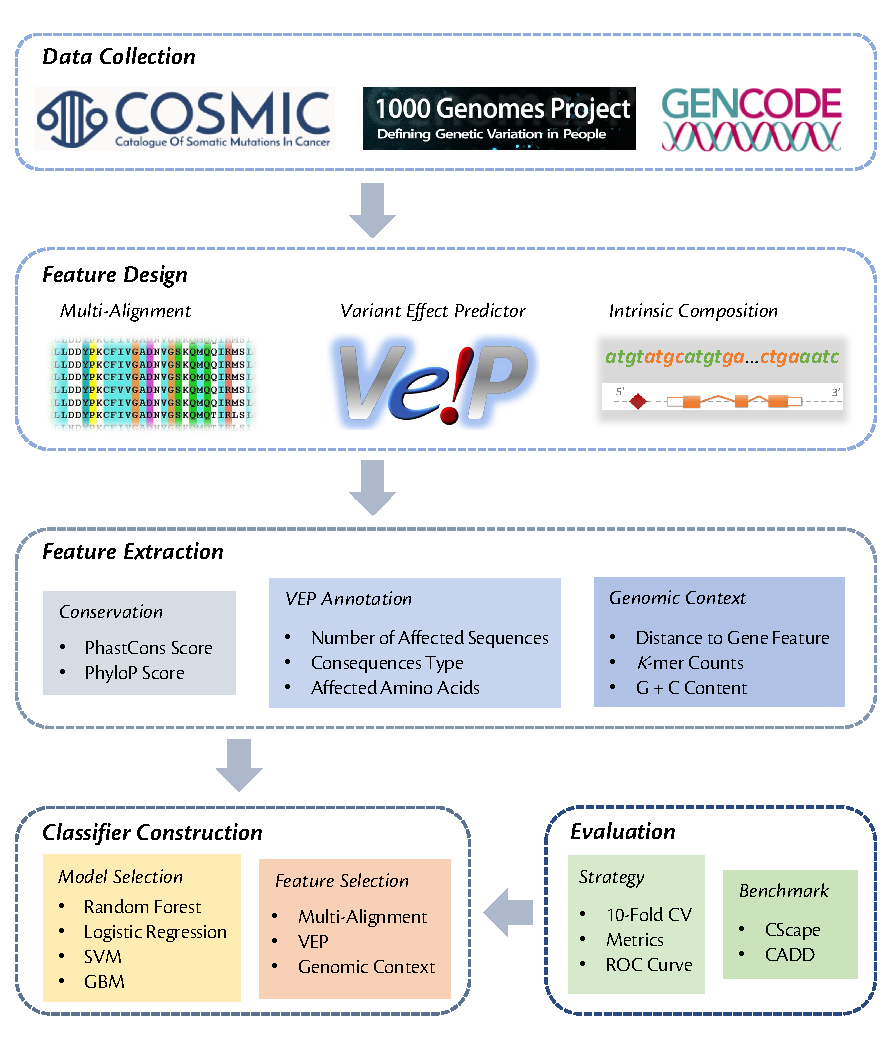
\includegraphics[width=\linewidth]{Framework.pdf}%

  \stepcounter{figure}
  \smallskip\noindent\small Figure \thefigure:
Framework of this study. %
  \label{fig:framework}%
\end{figure*}

\clearpage
\chapter{Data Collection}

The latest version of reference genome assembly is GRCh38. To ensure both the positive and negative variants are identified from the same reference genome, the variants used in this study are collected from the latest release of variant sets. Oncogenic variants are collected from database COSMIC (v89, release 15, May 2019), while neutral variants are collected from 1000 Genomes Project (release date: 31 May 2018). The reference alleles of both source data are compared to ensure the reference alleles at the same position are identical.

\begin{figure*}[b!]
  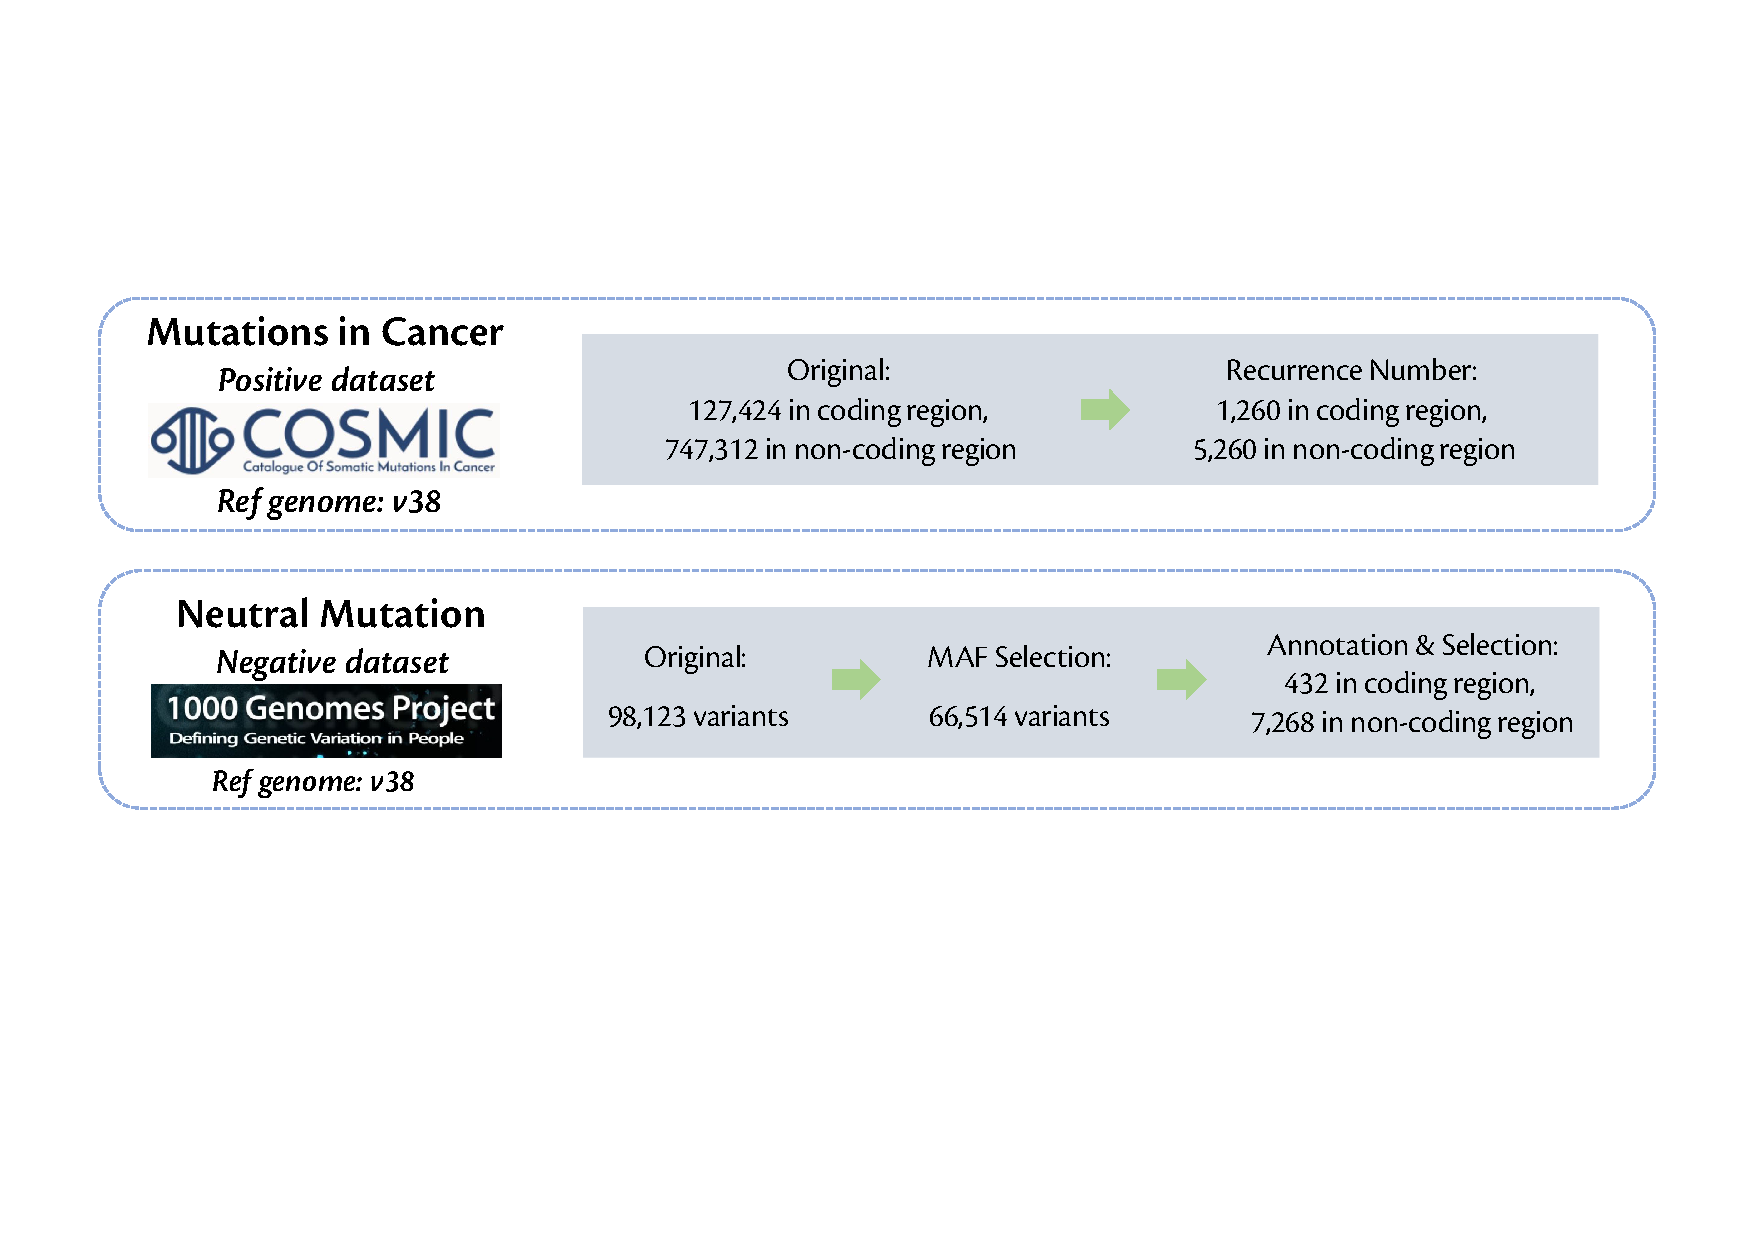
\includegraphics[width=\linewidth]{DataProcess.pdf}%

  \stepcounter{figure}
  \smallskip\noindent\small Figure \thefigure:
Illustration of data pre-processing. For COSMIC database, only those variants reach recurrence level (5 for coding region while 4 for non-coding region) will be selected to construct dataset. Neutral variants in 1000 Genomes Project are first filtered by their global minor allele frequency (MAF) values. Variants whose MAF is less than 1\% are further mapped onto human genome annotation file. And only those neutral mutations located within the flanks of 1,000 nt of the positive mutations will be kept.
  \label{fig:dataset}%
\end{figure*}

\begin{figure*}[t]
  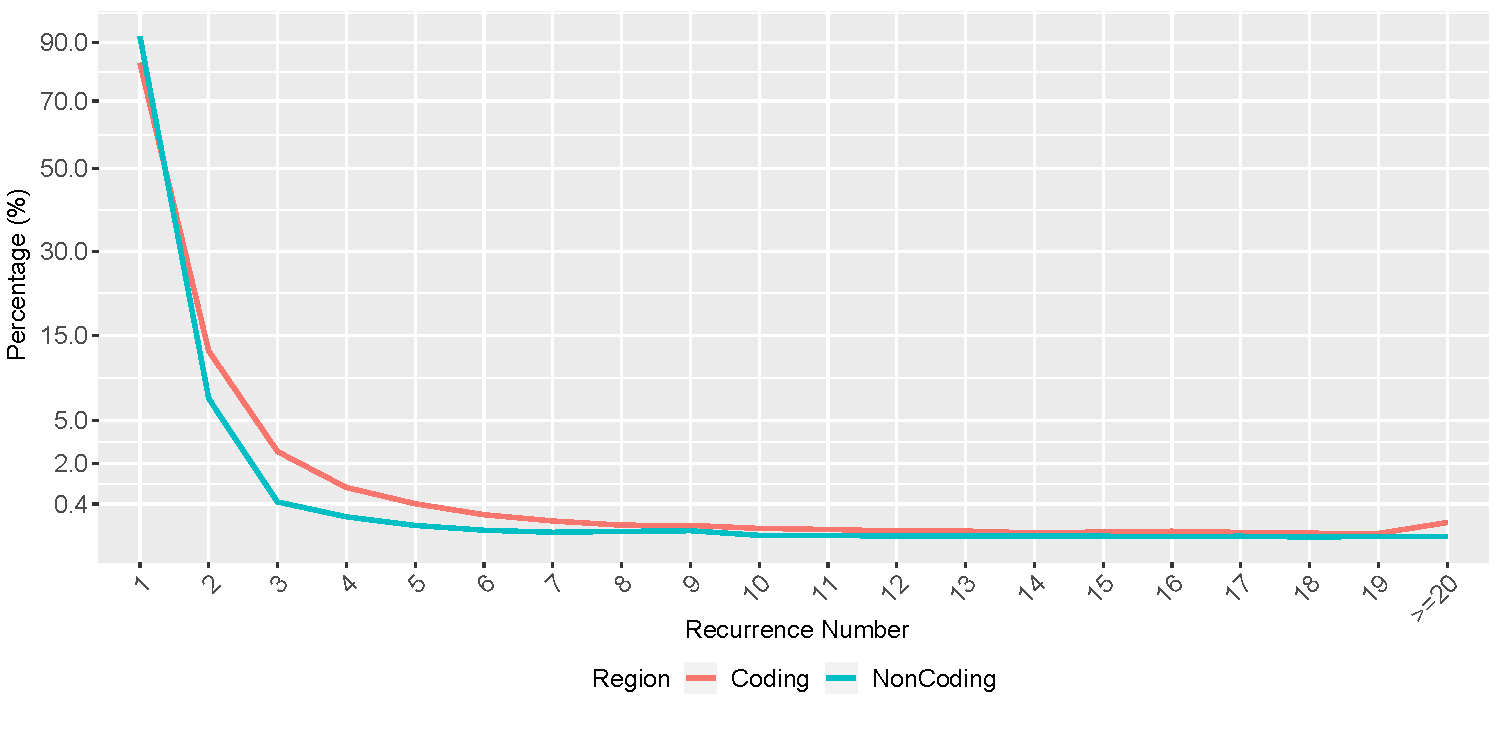
\includegraphics[width=\linewidth]{RecurrenceNumber.pdf}%

  \stepcounter{figure}
  \smallskip\noindent\small Figure \thefigure:
The percentage of variants (from COSMIC database) at different recurrence level.
  \label{fig:recurrenceNum}%
\end{figure*}

Data from COSMIC and 1000 Genomes Projects are pre-processed to build a gold standard dataset and minimise potential bias in predictor development (see Figure 5.1). As discussed in Introduction section, coding and non-coding regions in genome serve significantly different functions in biological process, and some properties are not applicable to both regions. Thus, it is sensible to build classifiers for coding and non-coding variants, respectively.

In current release of COSMIC database, there are 127,424 and 747,312 variants in coding and non-coding regions, respectively. To boost the confidence that the variants from COSMIC are not produced by chance, recurrence number, which is the number of times that a mutation has been observed in different samples, is used as a criterion to find reliable putative oncogenic variants. If we set a high threshold for recurrence number, we are more likely to obtain some variants that are widely existed in tumour, but the number of examples in dataset drops dramatically (see Figure 5.2). Experimental results proved that recurrence number $\geqslant$ 5 for variants in coding region and $\geqslant$ 3 for variants in non-coding region strikes the best balance between accuracy and data sufficiency. After applying this threshold to COSMIC dataset, 1,260 and 5,260 variants from coding and non-coding regions are selected to construct positive dataset.

\begin{table}[b]
        \begin{center}
        \begin{tabular}{ccc}
        \toprule
         \multirow{2}{*}{\textbf{Region}} & \multicolumn{2}{c}{Dataset} \\
        \cmidrule(l){2-3}
         & Training and validation set & Test set \\
        \midrule
    Coding     & 346 (positive) + 346 (negative)     & 86 (positive) + 86 (negative)     \\
    Non-coding & 4,208 (positive) + 4,208 (negative) & 1,052 (positive) + 1,052 (negative)  \\
        \bottomrule
        \end{tabular}
        \end{center}
    \caption{Overview of datasets used in this study}
    \label{tab:dataset}
\end{table}

For variants in 1000 Genomes Project, we first remove those SNVs that are present in pathogenic dataset and then select the SNVs whose global minor allele frequency $\leqslant$1\%. Unlike variants in COSMIC database, variants in 1000 Genomes Project have not been identified as coding variants or non-coding variants. To determine the variants are from coding or non-coding regions, variants in 1000 Genomes Project are first mapped onto genome annotation file (version GRCh38 patch13) downloaded from GENCODE. However, each gene has six different open reading frame (ORF), and each ORF may contain several different transcripts. According to the results from annotation file, we found that one variant can be simultaneously located in both coding and non-coding transcripts. To build a reliable dataset, we further use VEP to calculate amino acids substitution introduced by the single point mutations. If one reference allele involves no amino acid, the mutations at this point are regarded as non-coding mutations. Studies proved that if the negative variants are too far away from the positive variants in genome, bias can be introduced, which makes the final prediction results too optimistic. To avoid this bias, only those neutral mutations located within the flanks of 1000 nt of the positive mutations will be selected to build negative datasets. We finally obtain 432 coding variants and 7,268 non-coding variants from 1000 Genome Project.

To create balance datasets, 432 coding variants 5,260 non-coding variants are randomly selected from COSMIC and 1000 Genomes Projects, respectively. Then about 20\% variants of each region are randomly selected to construct test set, and the remaining variants serve as training set and validation set for 10-fold CV. Datasets used in this study are summarised in Table \ref{tab:dataset}.

\clearpage
\chapter{Feature Engineering}

In this study, the discriminating power of three kinds of feature categories: evolutionary conservation, VEP results and genomic context information are discussed and evaluated.

Evolutionary conservation contains conservation scores to evaluate if the mutations are located in some highly conserved sites. VEP can give comprehensive summarise, such as pathogenicity scores, co-located variants, position of CDS (coding sequence) affected by the mutations, of the input variants. Only the results that can reflect the genuine information of the mutations will be used to design features. Genomic context-based features are designed to show the sequence intrinsic context of the variants. The design and extraction of these features will be elaborated in this chapter.


\section{Evolutionary Conservation}

Mutations in conserved regions tend to have greater impacts than those in non-conserved regions. A slight modification in highly conserved genes can cause critical functional disorder of organisms. Here we use 30- and 100-Way PhastCons and phyloP scores provided by UCSC genome browser to describe the conservation level of each position in human genome. 30-Way scores are calculated by aligning human genome against 29 mammalian genomes, while 100-Way scores are obtained by aligning against 99 vertebrate genomes.

\section{VEP Annotation}

\begin{figure*}[t]
  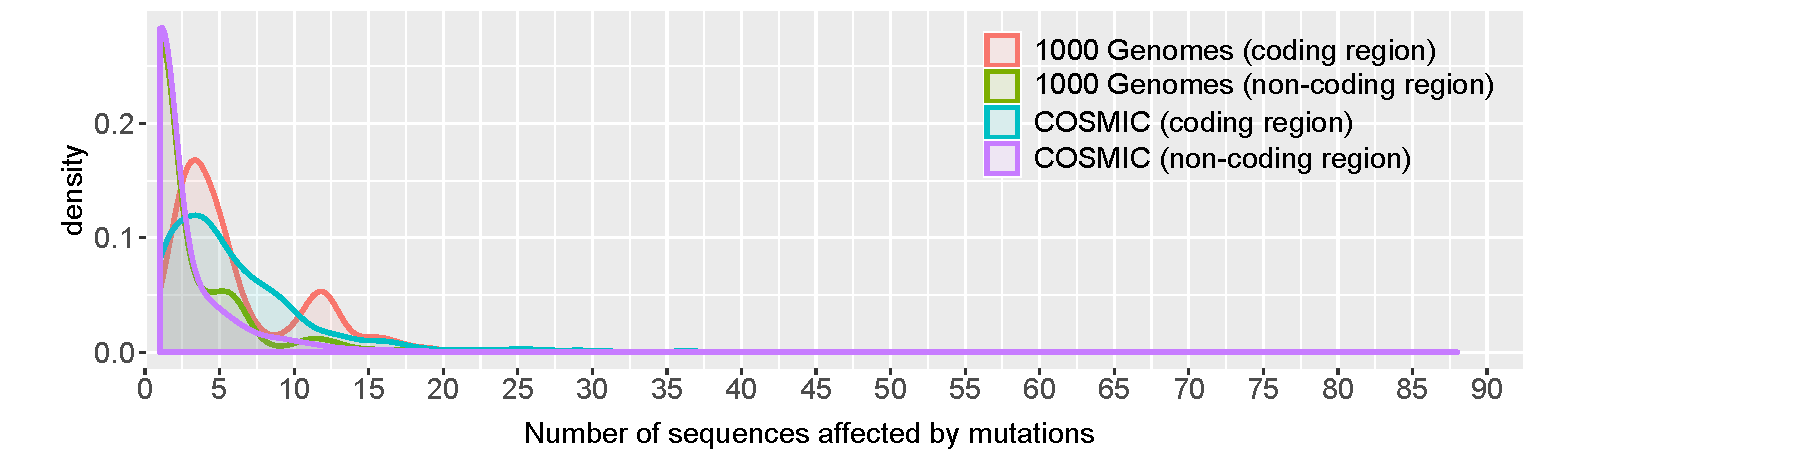
\includegraphics[width=\linewidth]{dist_vepNum.pdf}%

  \stepcounter{figure}
  \smallskip\noindent\small Figure \thefigure:
Density plot of number of sequences affected by mutations.
  \label{fig:dist_vepNum}%
\end{figure*}

\begin{figure*}[b!]
  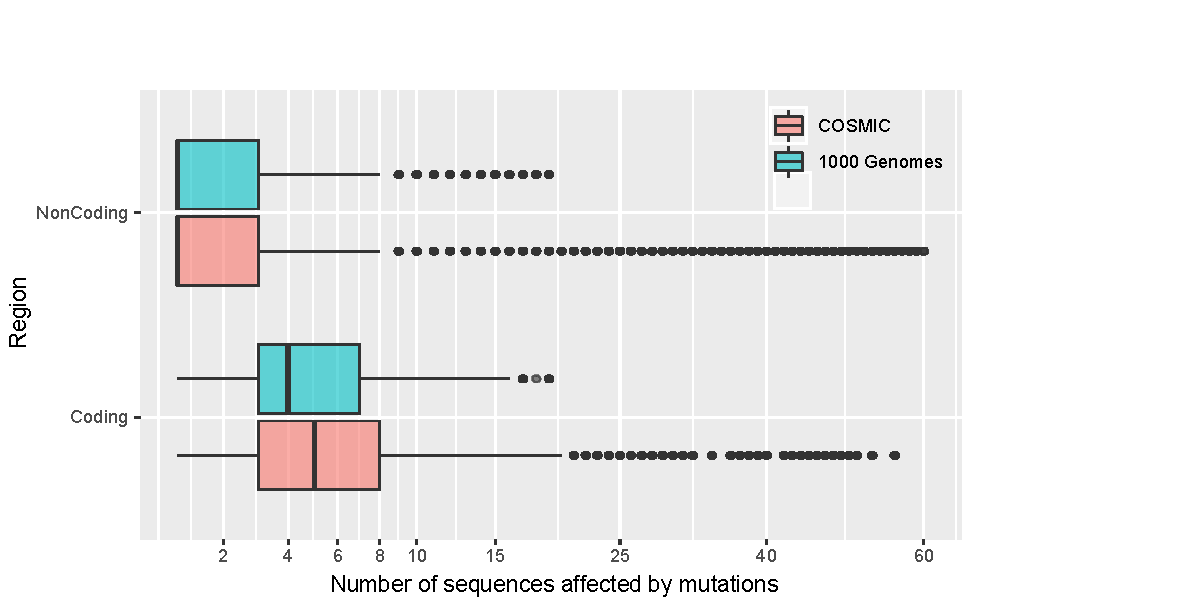
\includegraphics[width=\linewidth]{vepNum.pdf}%

  \stepcounter{figure}
  \smallskip\noindent\small Figure \thefigure:
Overview of number of sequences affected by mutations. Positive mutations (from COSMIC) tend to affect more transcripts or genes than neutral mutations (from 1000 Genomes Project). A scale transformation has been added to the x-axis to improve the visual appearance.
  \label{fig:vepNum}%
\end{figure*}

\begin{table}[tp]
  \begin{center}
    % \footnotesize%
    \begin{tabular}{lll}
      \toprule
3' prime UTR$^1$ variant              & mature miRNA variant       & start lost               \\
5' prime UTR variant               & missense variant           & start retained variant   \\
coding sequence variant            & NMD$^2$ transcript variant    & stop gained              \\
downstream gene variant            & in-frame deletion          & stop lost                \\
feature elongation                 & in-frame insertion         & stop retained variant    \\
feature truncation                 & protein altering variant   & synonymous variant       \\
frameshift variant                 & regulatory region ablation & TF$^3$ binding site variant \\
incomplete terminal codon variant  & intron variant             & TFBS$^4$ ablation           \\
non-coding transcript exon variant & regulatory region variant  & TFBS amplification       \\
non-coding transcript variant      & splice acceptor variant    & transcript ablation      \\
intergenic variant                 & splice donor variant       & transcript amplification \\
regulatory region amplification    & splice region variant      & upstream gene variant  \\
      \bottomrule
    \end{tabular}
  \end{center}
  \caption{The set of consequence terms provided by VEP. The variants are mapped to the reference genome, and each allele of each variant may have a different effect in different transcripts.\\
$^1$untranslated region; $^2$Nonsense-mediated mRNA decay; $^3$transcription factor; $^4$transcription factor binding site
}
  \label{tab:vepCons}
\end{table}

\begin{figure*}[bp]
  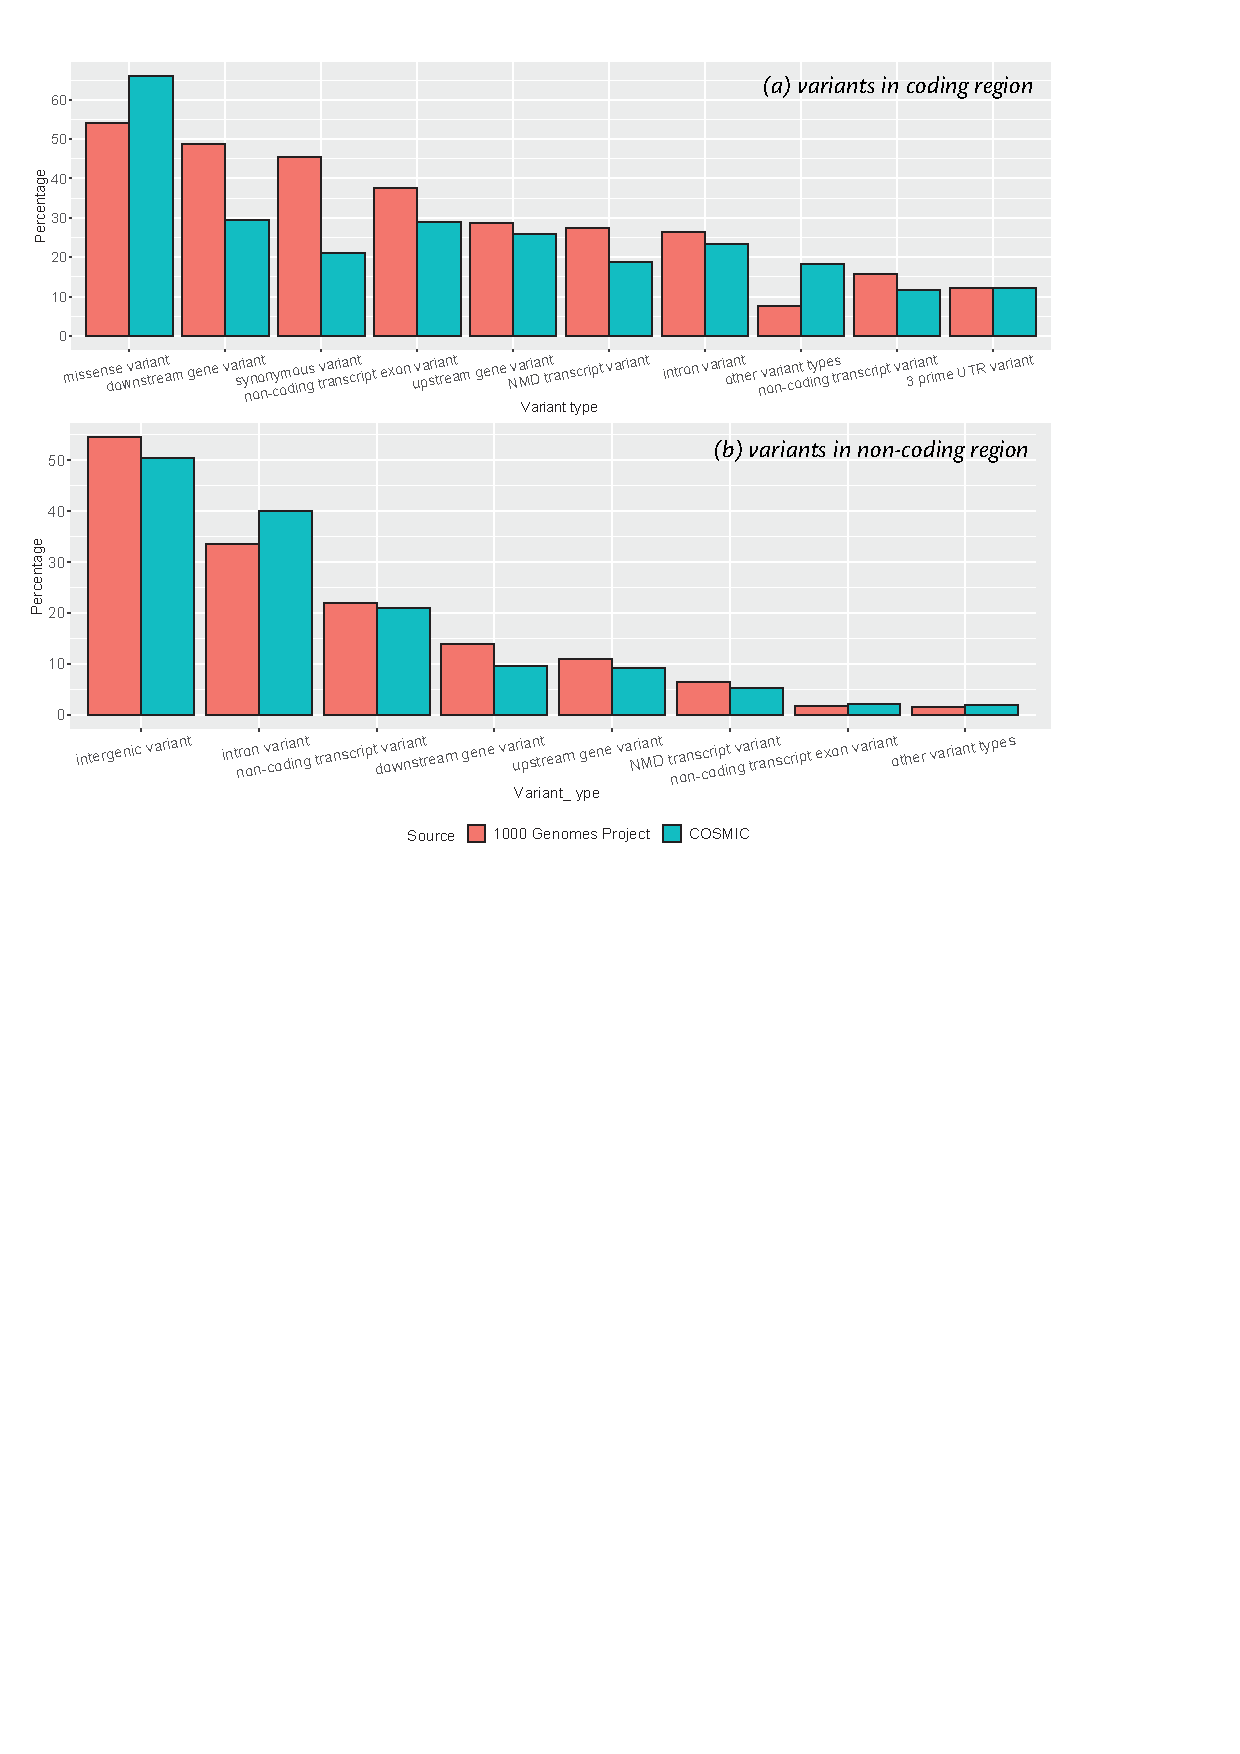
\includegraphics[width=\linewidth]{summary_vep_cons.pdf}%

  \stepcounter{figure}
  \smallskip\noindent\small Figure \thefigure:
Distribution of variant consequence produced by Variant Effect Predictor (VEP). Pathogenic and neutral variants in coding and non-coding region lead to different types of variant consequences.
  \label{fig:vepCons}%
\end{figure*}

Three kinds of features can be extracted from VEP's annotation: the \textbf{Num}ber of transcripts affected by the variants (vepNum), the \textbf{Cons}equence types of the variants (vepCons) and the \textbf{A}mino \textbf{A}cid substitution caused by the variants (vepAA).

The alterations of some nucleotides may affect multiple transcripts, and further affect some biological functions. Figure 6.1 shows the density of the number of sequences affected by the variants from coding and non-coding region. The boxplot in Figure 6.2 also shows the distribution of vepNum. All variants from COSMIC and 1000 Genomes Project are included into our analysis. Although vepNum of positive and negative variants present similar distribution, we can still notice that positive variants have more outliers (see Figure 6.2) and tend to affect more transcripts than neutral mutations.

vepCons means the changes to associated transcripts. For example, a mutation located in UTR (untranslated region) may cause "3' prime UTR variant" or "5' prime UTR variant". Currently, variants are categorised into 36 consequence types (see Table \ref{tab:vepCons}), but the top 10 consequence types have encompassed the majority of variants in X chromosome (see Figure 6.3). For example, in coding region, 66.02\% positive variants and 54.09\% negative variants can cause consequence missense variant; in non-coding region, 50.39\% positive variants and 54.49\% negative variants are related to consequence intergenic variant. Please note that  one mutation can simultaneously cause multiple consequences. In this research, we use 36 binary vectors (one vector per consequence type) to represent the consequence(s) of one variant.

Features of vepAA are designed to record the alterations of amino acids caused by the single point mutation. One variant can be simultaneously located in several different transcripts, and based on different ORFs, one variant can change several amino acids. To capture the change in amino acid composition, two sets of feature vectors will be used to reflect the reference and mutated residues, respectively. Each set contains 20 binary vectors (one vector per amino acid type) to represent the amino acid conditions.

\section{Genomic Context Information}

Features in genomic context feature group can be further divided into three subgroups: distance scores, G + C content and \emph{k}-mer features.

Distance scores are used to evaluate the distance between different gene features and the mutations. Information of seven types of gene features (gene, transcript, UTR, CDS, start codon, stop codon and exon) is collected from the genome annotation file provided by GENCODE. And the distance scores are computed by measuring the distance between the variant and the nearest example of each gene feature. To better capture the connections between variants and gene features, distance is only computed when gene feature is located within a window of \emph{w} nt around the mutations. Then distance will be mapped onto the range [0, 1] using following equation:

\begin{equation}
    \text{Distance score} = \left\{
    \begin{array}{ll}
        \frac{1}{d + 1} ,               & d $\leqslant$ w \\
        \text{0} , & \text{otherwise}}
    \end{array}
    \right. , \nonumber
\end{equation}

\noindent where \emph{d} is the distance between variant and its nearest example of each gene feature. Using this strategy, seven distance scores (one vector per gene feature) can be extracted. The optimum \emph{w} will determined with experiments. In this study, different \emph{w} from range [1, 100,000] are evaluated.

G + C content and \emph{k}-mer features are used to measure the alteration of sequence intrinsic composition around the mutation. Given a mutation and its flanking sequences, we calculate two sets of G + C content and \emph{k}-mer features which represents the genomic context around reference and mutated nucleotides. Two parameters need to be determined for these two kinds features: \emph{w} of window width and \emph{k} of \emph{k}-mer patterns. There are also two strategies to capture \emph{k}-mer information: \emph{k}-mer counts and \emph{k}-mer frequencies. \emph{K}-mer frequencies are calculated using:

\begin{equation}
    f_i = \frac{c_i}{s_k}, \quad i = 1, 2, 3, ..., \sum_{n = 1}^{k}{4^n},
     \nonumber
\end{equation}

\begin{equation}
    s_k = w - k + 1,
     \nonumber
\end{equation}

\noindent where $f_i$ is the frequency of the \emph{i}th \emph{k}-mer pattern and $c_i$ is the count of the \emph{i}th \emph{k}-mer pattern; \emph{w} is the length of window, and thus $s_k$ denotes the total number of \emph{k}-mer patterns in the window. For a single point mutation, we hope to confine the window width into a relatively small range around the mutation. In this sudy, we perform grid search to find the optimum \emph{w} and \emph{k} within the range \emph{w} $\in$ \{1, 3, 5, 7, 9\}, \emph{k} $\in$ \{1, 2, 3, 4\}.

\chapter{Feature Selection and Model Construction}

Sequential learning strategy is used to identify the best feature combination. We first combine different feature groups with the best feature and build random forest classifiers using training and validation sets. The classifier will be tuned with 10-fold CV and used to predict the variants in test set. Based on the statistics obtained from the prediction, we can obtain the two top-ranked feature groups. Then subsequent models will be built by adding other feature groups in descending order of accuracy, and we determine the three top-ranked feature groups. After evaluating all possible feature combinations, we select the feature combination that achieves the highest accuracy as the final combination.

After obtaining the optimum feature combinations, these features will be incorporated into logistic regression, SVM and GBM classifiers. Parameters of these classifiers will be tuned using 10-fold CV and grid search. The model achieving the highest accuracy will be selected to build CScape-X.

The computational speed will be evaluated in terms of the extraction of different feature groups, model training and variant prediction.

\part{Results, Analyses and Summary}

\chapter{Results}

The evaluation results are summarised in this chapter. Different feature groups and feature combinations are first evaluated with random forest. After determining the optimal feature combinations, three other machine learning methods, logistic regression, SVM and GBM, are used to build the classifier. The method that achieves the highest accuracy will be finally selected to build CScape-X. CScape-X is then benchmarked against two existing tools, its precursor CScape and widely-used tool CADD. An analysis on computational speed is finally carried out to evaluate the efficiency of CScape-X.

For every evaluation of features and machine learning methods, we first use training sets and validation sets to perform 10-fold CV and parameter tuning, then a fine-tuned classifier will be trained. The final performance is obtained from an independent test set. The performances are evaluated with ROC curve and five standard statistics: sensitivity, specificity, accuracy, F-measure, and Kappa Coefficient \cite{Cohen1960}.

\begin{equation}
    \text{Sensitivity} = \frac{TP}{TP+FN} , \quad
    \text{Specificity} = \frac{TN}{TN+FP} , \nonumber\\
\end{equation}
% \vspace*{2pt}

\begin{equation}
    \text{Accuracy} = \frac{TP+TN}{P+N} , \quad
    \text{Kappa} = \frac{Pr(o)-Pr(e)}{1-Pr(e)} , \nonumber\\
\end{equation}
% \vspace*{2pt}

\begin{equation}
    \text{F-Measure} = \frac{2 \times TP}{2 \times TP+FP+FN} .\nonumber\\
\end{equation}
\vspace*{2pt}

In Cohen's Kappa Coefficient, \text{\it Pr(o)} denotes the proportion of units in which the judges agreed, and \text{\it Pr(e)} is the proportion of units for which agreement is expected by chance. Kappa value can measure inter-rater reliability for classification problem. Equally arbitrary guidelines \cite{Fleiss2003} characterise kappa over 0.75 as excellent, 0.40 to 0.75 as fair to good, and below 0.40 as poor.

\section{Feature Evaluation}

\begin{figure*}[tb]
  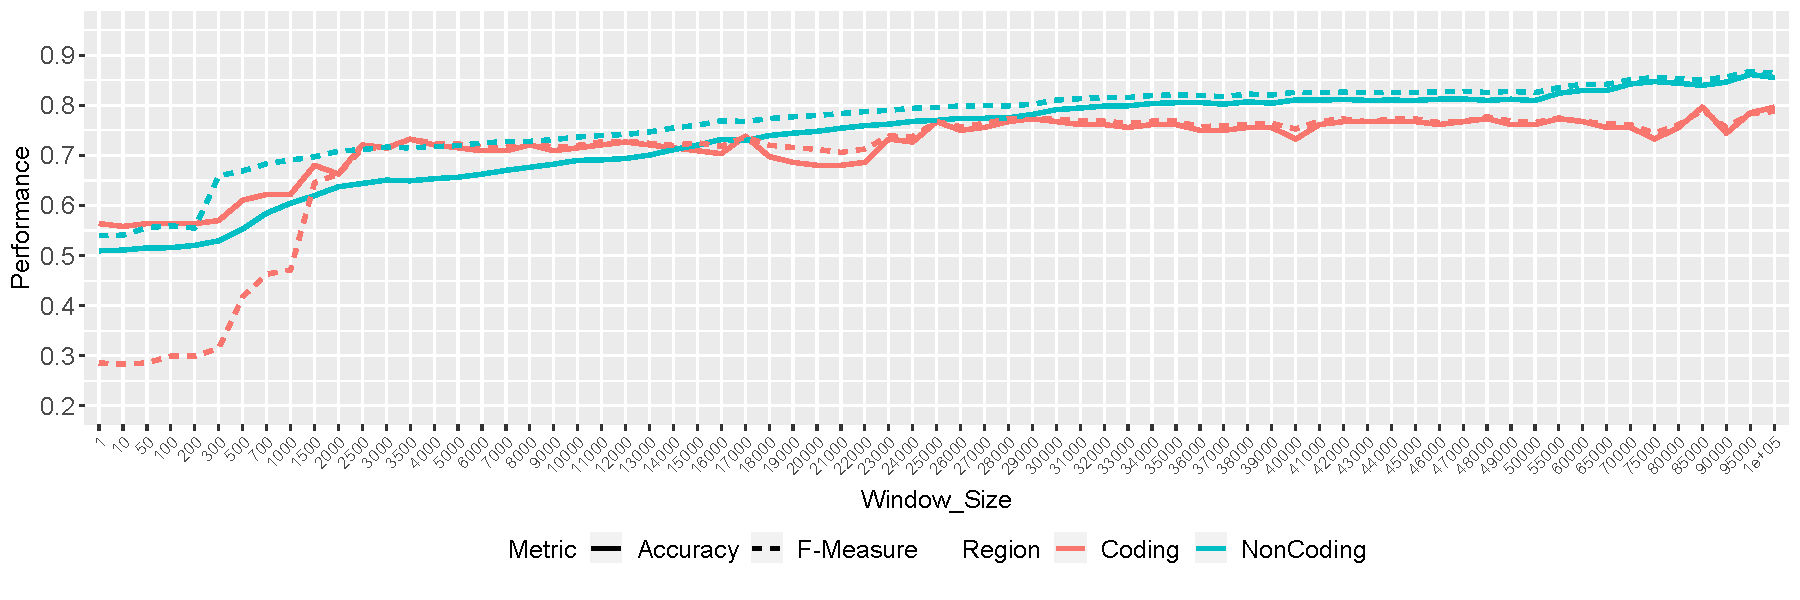
\includegraphics[width=\linewidth]{perf_distance.pdf}%

  \stepcounter{figure}
  \smallskip\noindent\small Figure \thefigure:
Performance of distance-derived feature group (distance to the nearest gene feature) under different window sizes (from 1 to 100,000 nt). The best performance of coding model (accuracy: 0.7965, F-measure: 0.7904) occurs when the width is 85,000 nt; while the optimal width for non-coding model is 95,000 (accuracy: 0.8617, F-measure: 0.8679). Accuracy and F-measure in the figure are calculated on test set using random forest classifier. Parameters of the classifier have been tuned on training and validation set with 10-fold CV. %
  \label{fig:dist}%
\end{figure*}

\begin{figure*}[b!]
  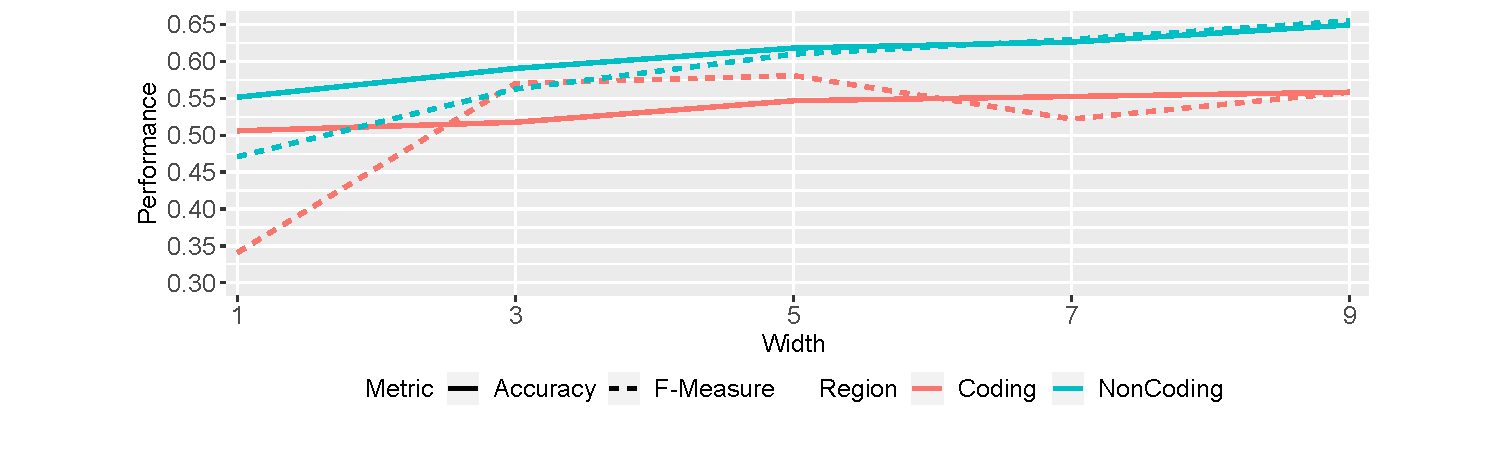
\includegraphics[width=\linewidth]{perf_gc.pdf}%

  \stepcounter{figure}
  \smallskip\noindent\small Figure \thefigure:
Performance of G + C content under different window sizes (from 1 to 9). The optimal width is 9 nt for both coding and non-coding models. The highest accuracy of coding model is 0.5581; the highest accuracy of non-coding model is 0.6492. Accuracy and F-measure in the figure are calculated on test set using random forest classifier. Parameters of the classifier have been tuned on training and validation set with 10-fold CV. %
  \label{fig:gc}%
\end{figure*}

Features from three feature groups, multiple alignment-based conservation score, VEP results and genome context information, are used to construct method CScape-X. Before building classifier for oncogenic SNV prediction, different features should be comprehensive evaluated. Here we first determine the optimal window width \emph{w} and \emph{k} for the features in genome context feature group.

We assess the performance of distance-based features under different window widths by constructing random forest classifier using training and validation sets, and the classifier will be evaluated using independent test set. The window widths range from 1 nt to 100,000 nt. The results are shown in Figure 7.1. With increasing of window width, the accuracy and F-measure of non-coding model improves steadily. Performance of coding model, however, shows some fluctuations. Non-coding model achieves the best performance, accuracy of 0.8617 and F-measure of 0.8679, when window width is 95,000 nt; Coding model obtains the highest accuracy 0.7965 and F-measure 0.7904 when width equals 85,000 nt. Thus, distance score is calculated within 85,000 nt and 95,000 nt windows for SNVs in coding and non-coding region, respectively.

\begin{figure*}[t]
  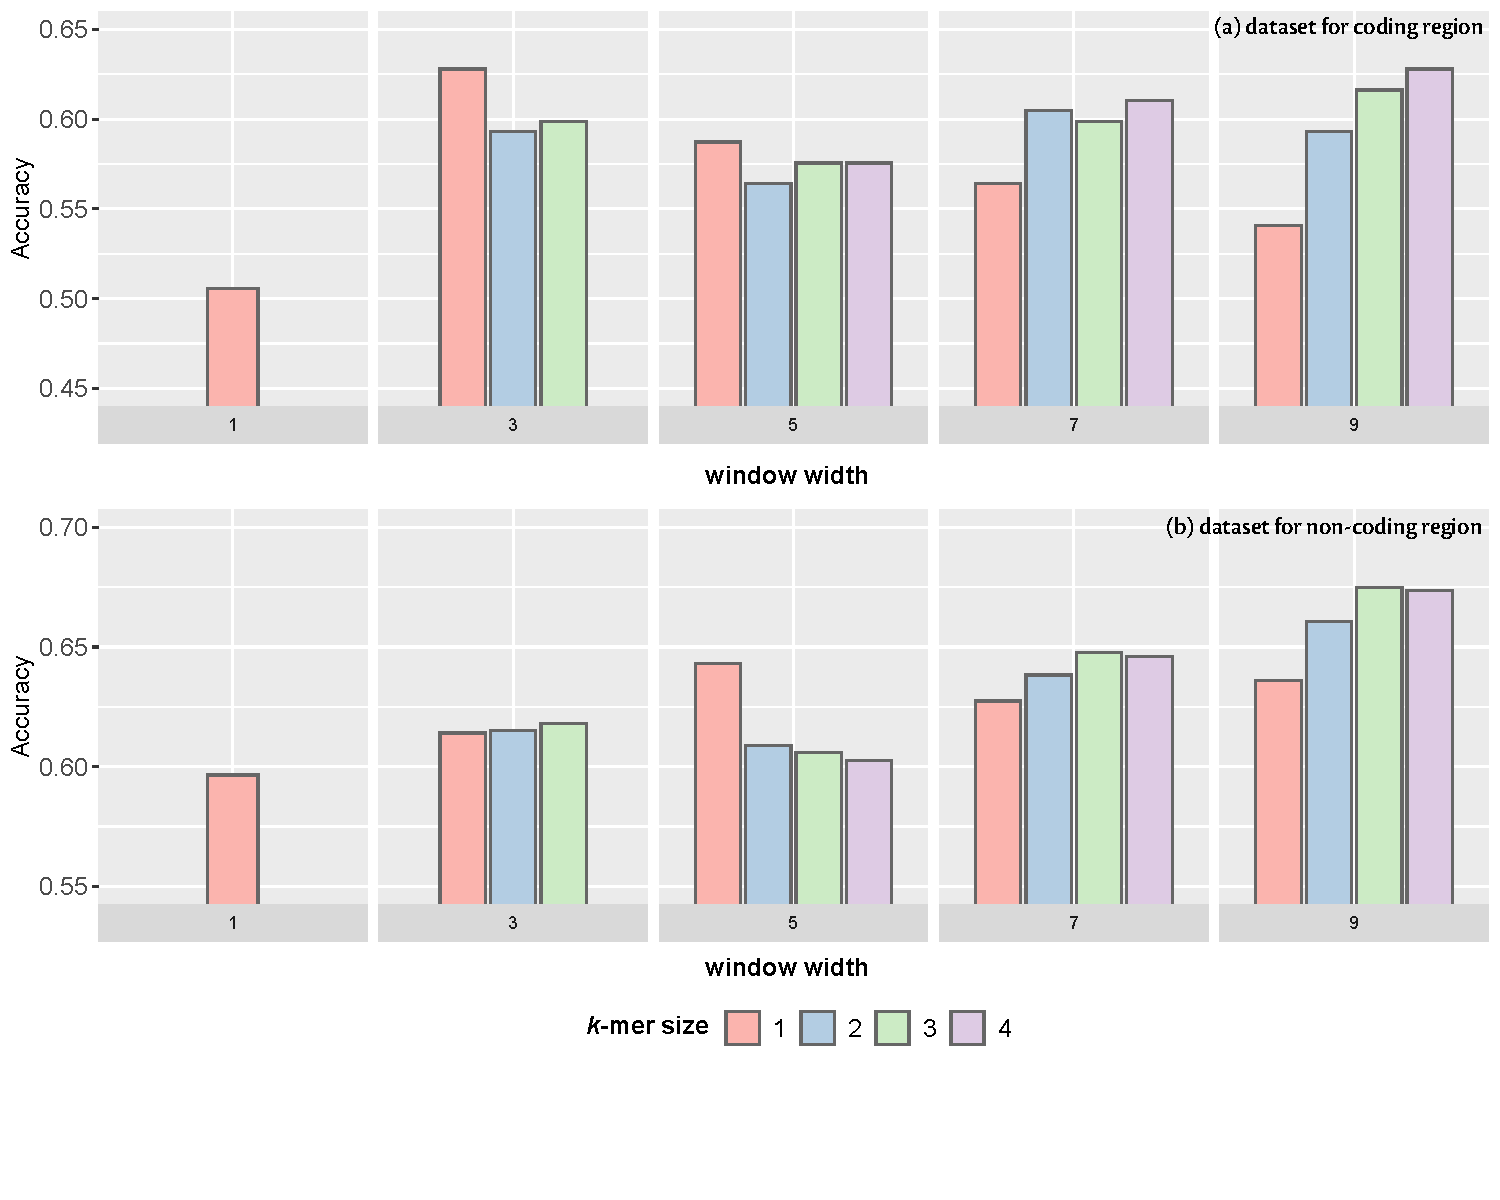
\includegraphics[width=\linewidth]{perf_spectrum_num.pdf}%

  \stepcounter{figure}
  \smallskip\noindent\small Figure \thefigure:
Accuracy of \emph{k}-mer count feature group under different \emph{k} (from 1 to 4) and window sizes (from 1 to 9). The optimal combination for coding model is 1-mer counts on 3 nt sub-sequence (accuracy: 0.6279). For non-coding models, the highest accuracy is 0.6749 when calculating 3-mer counts on 9 nt sub-sequence. Accuracy is calculated on test set using random forest classifier. Parameters of the classifier have been tuned on training and validation set with 10-fold CV.  %
  \label{fig:kmer_count}%
\end{figure*}

\begin{figure*}[t]
  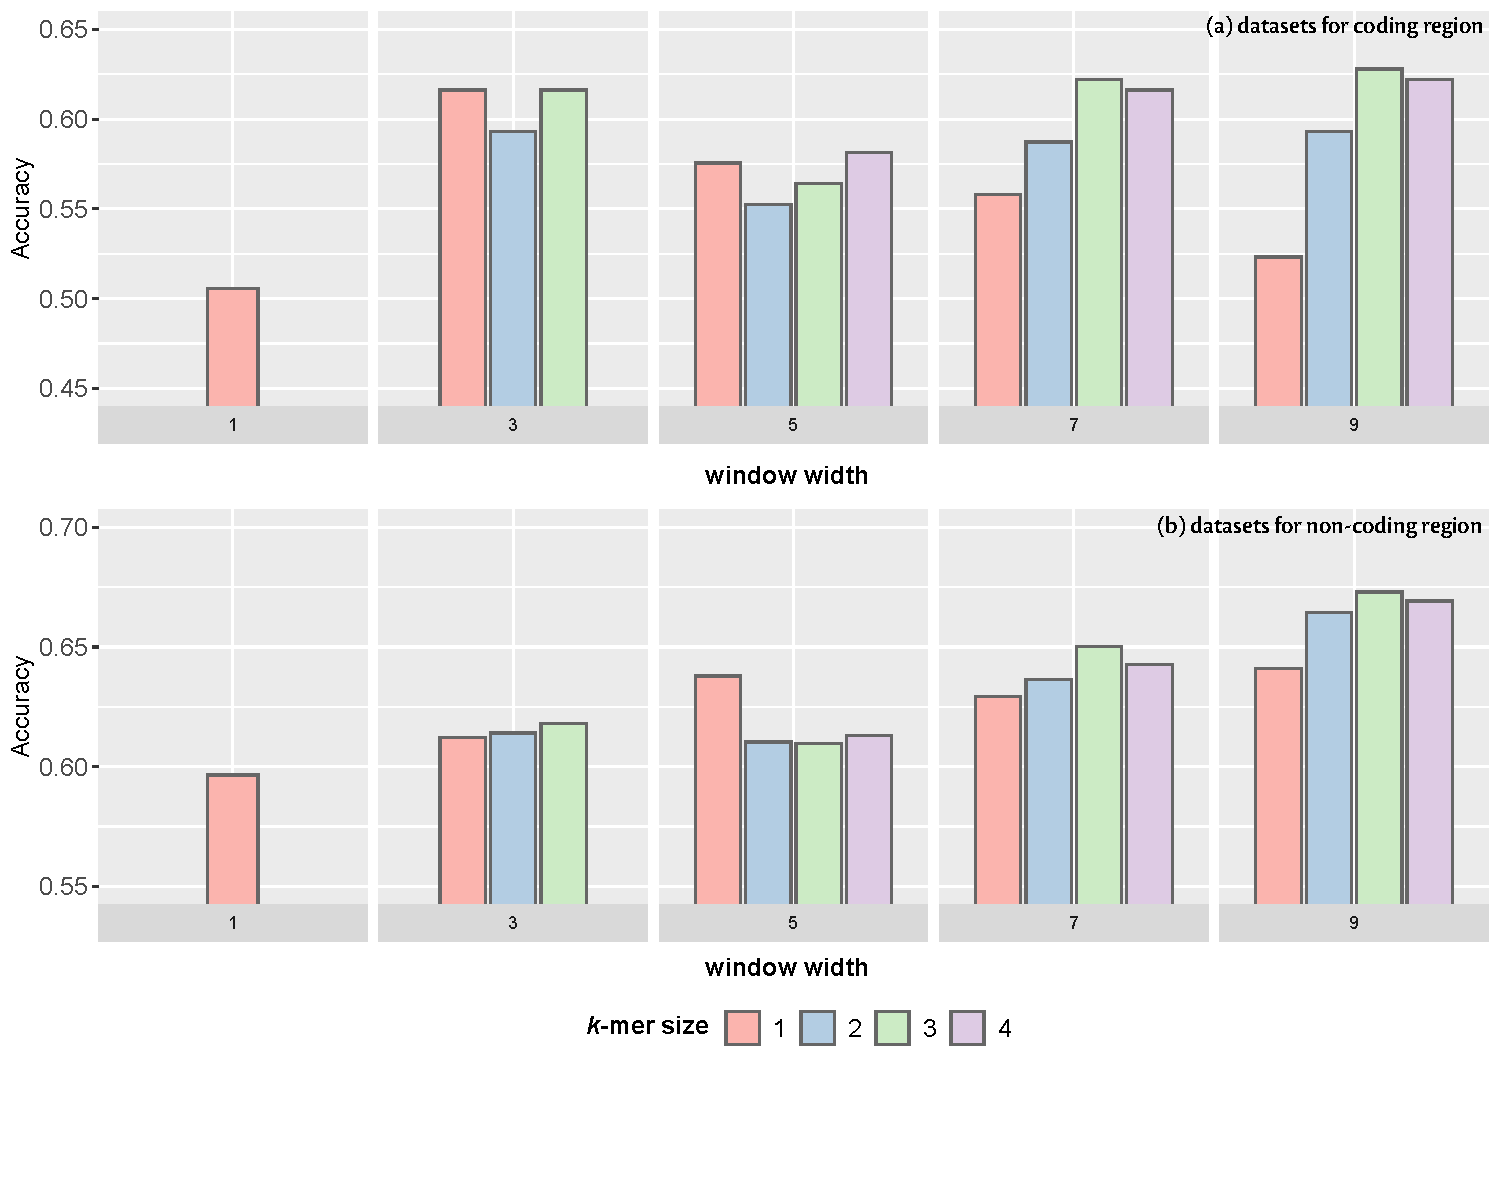
\includegraphics[width=\linewidth]{perf_spectrum_freq.pdf}%

  \stepcounter{figure}
  \smallskip\noindent\small Figure \thefigure:
Performance of \emph{k}-mer frequencies feature group under different \emph{k} (from 1 to 4) and window sizes (from 1 to 9). The optimal combination for coding and non-coding model is 3-mer counts on 9 nt sub-sequence, which achieves accuracy 0.6279 for variants from coding region and accuracy 0.6730 for variants from non-coding region. Accuracy is calculated on test set using random forest classifier. Parameters of the classifier have been tuned on training and validation set with 10-fold CV.  %
  \label{fig:kmer_freq}%
\end{figure*}

We further used similar method to determine the optimal width of G + C content. We established five different window widths (1, 3, 5, 7 and 9 nt) with the centre of mutated point. And G + C content was calculated on these sub-sequences. The results are displayed in Figure 7.2. Both the coding and non-coding models obtain best results when width is 9 nt. In this case, model for coding region achieves accuracy and F-measure of 0.5581, while model for non-coding region achieves accuracy 0.6492 and F-measure 0.6548. Hence, G + C content is computed on 9 nt sub-sequence with the centre of mutated site.

\emph{K}-mer information is captured with \emph{k}-mer counts and frequencies under different window widths and \emph{k}. For \emph{k}-mer features, \emph{k} ranges from 1 to 4, and window widths include 1, 3, 5, 7 and 9 nt. The results of \emph{k}-mer counts and frequencies are displayed in Figure 7.3 and Figure 7.4, respectively. The differences in results between \emph{k}-mer frequencies and counts are minor. For coding model, both \emph{k}-mer counts and frequencies obtain accuracy 0.6279, but the optimal combination of \emph{k}-mer counts is \emph{k} = 1 and width = 3, and the optimal combination of \emph{k}-mer frequencies is \emph{k} = 3 and width = 9; for non-coding model, both \emph{k}-mer counts and frequencies features achieve the highest accuracy when calculating 3-mer on 9 nt sub-sequence: 0.6749 for \emph{k}-mer counts and 0.6730 for \emph{k}-mer frequencies. Comparing the performances of two kinds of feature extraction strategies, 1-mer counts on 3 nt and 3-mer counts on 9 nt sub-sequences are selected as candidate feature groups for coding and non-coding models, respectively.

After determining the optimal \emph{k} and width for genomic context-based features, all candidate features and feature groups have been determined. In following experiments, seven feature groups: conservation score, vepNum, vepCons, vepAA, G + C content, distance score and \emph{k}-mer counts are evaluated for variants in coding and non-coding regions separately.

\begin{table}[t]
  \begin{center}
    \footnotesize%
    \begin{tabular}{lrrrrr}
      \toprule
      Feature group & Sensitivity & Specificity & Accuracy & F-Measure & Kappa \\
      \midrule
      conservation       & 0.7326 & 0.7791 & 0.7558 & 0.7500 & 0.5116 \\
      distance           & 0.7907 & 0.7209 & 0.7558 & 0.7640 & 0.5116 \\
      vepCons   & 0.5233 & 0.8256 & 0.6744 & 0.6164 & 0.3488 \\
      G + C Content      & 0.5581 & 0.7093 & 0.6337 & 0.6038 & 0.2674 \\
      \emph{k}-mer              & 0.7093 & 0.5000 & 0.6047 & 0.6421 & 0.2093 \\
      vepNum & 0.5581 & 0.5581 & 0.5581 & 0.5581 & 0.1163 \\
      vepAA    & 0.4302 & 0.6395 & 0.5349 & 0.4805 & 0.0698 \\
      \bottomrule
    \end{tabular}
  \end{center}
  \caption{Performance of different feature groups evaluated on test set for coding region. Random forest classifier is built using training and validation set, and parameters are fine-tuned using 10-fold CV.}
  \label{tab:perf_fea_CD}
\end{table}

\begin{table}[t!]
  \begin{center}
    \footnotesize%
    \begin{tabular}{lrrrrr}
      \toprule
      Feature group & Sensitivity & Specificity & Accuracy & F-Measure & Kappa \\
      \midrule
    distance           & 0.9078 & 0.8165 & 0.8622 & 0.8682 & 0.7243 \\
    conservation       & 0.6369 & 0.7738 & 0.7053 & 0.6837 & 0.4106 \\
    \emph{k}-mer              & 0.6702 & 0.6606 & 0.6654 & 0.6670 & 0.3308 \\
    G + C Content      & 0.6949 & 0.6055 & 0.6502 & 0.6652 & 0.3004 \\
    vepNum & 0.7776 & 0.3897 & 0.5837 & 0.6513 & 0.1673 \\
    vepCons   & 0.7519 & 0.2947 & 0.5233 & 0.6120 & 0.0466 \\
      \bottomrule
    \end{tabular}
  \end{center}
  \caption{Performance of different feature groups evaluated on test set for non-coding region. Random forest classifier is built using training and validation set, and parameters are fine-tuned using 10-fold CV.}
  \label{tab:perf_fea_NC}
\end{table}

The performances of different feature groups on coding region and non-coding regions are shown in Table \ref{tab:perf_fea_CD} and \ref{tab:perf_fea_NC}. Conservation score and distance score achieve the highest accuracy. Only conservation scores or distance scores alone can generate acceptable accuracy $\sim$0.70, which reflects that these two features are relatively critical to pathogenic SNV prediction. Feature group vepCons yields passable results for variants in coding regions. Nonetheless, feature group vepCons gives the lowest accuracy for the prediction of oncogenic SNV in non-coding region. From the Figure 5.3, we can notice that the distributions of vepCons of SNVs in positive and negative datasets are very similar, and the majority of SNVs belong in consequence type "intergenic variant" or "intron variant", which may explain the weak performance of this feature group for non-coding region. The experiments of Table \ref{tab:perf_fea_CD} and \ref{tab:perf_fea_NC} are new evaluations for each feature group and independent of the experiments of Figure 7.1 to 7.4. Therefore, the same feature group may show different performances.

\begin{figure*}[tp]
  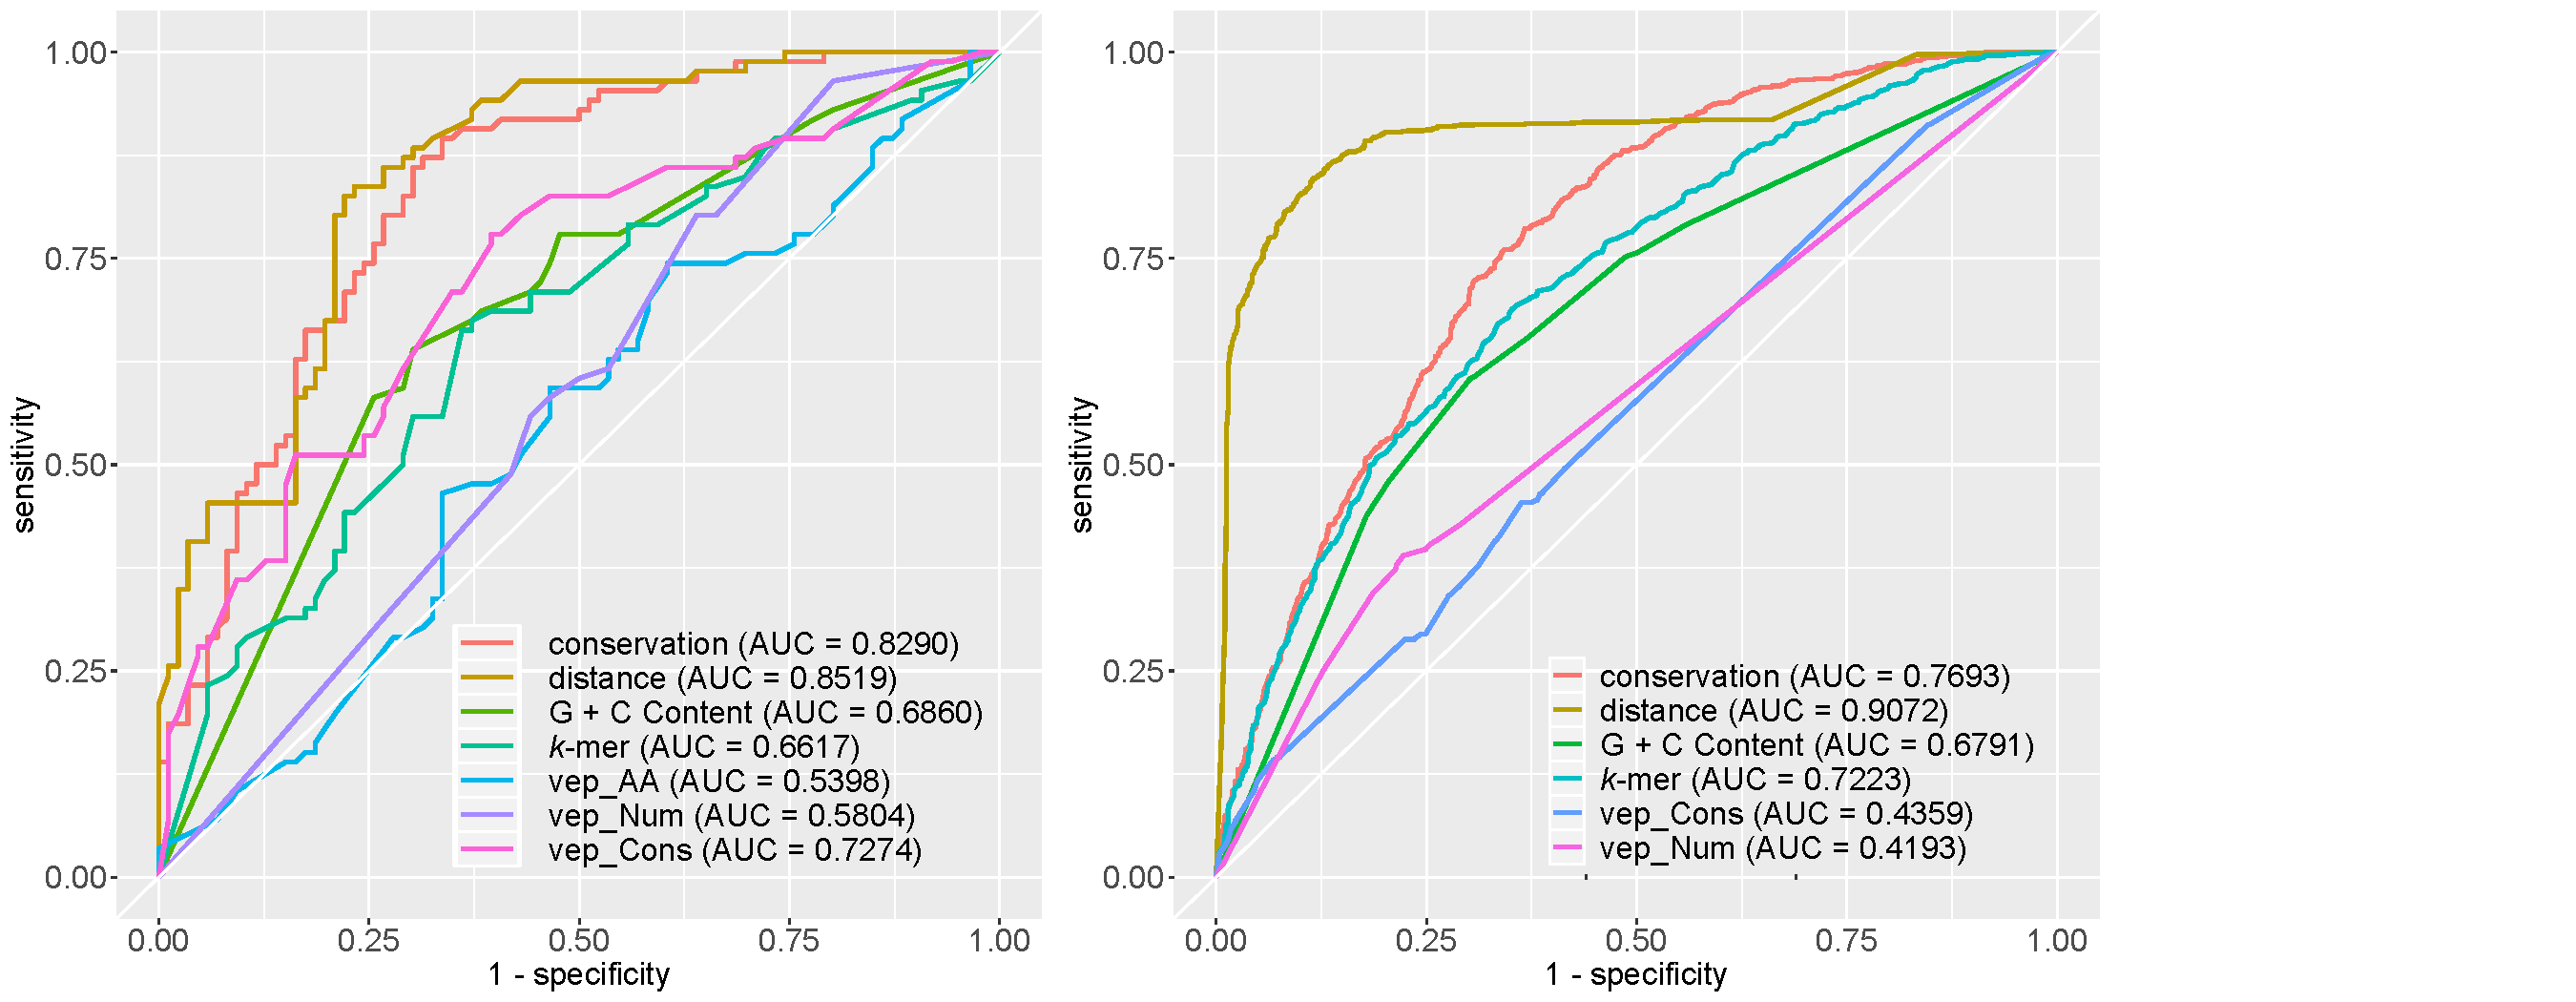
\includegraphics[width=\linewidth]{ROC_featureEval.pdf}%

  \stepcounter{figure}
  \smallskip\noindent\small Figure \thefigure:
   ROC curves of different feature groups for coding (left) and non-coding (right) regions.
  \label{fig:ROC_fea}%
\end{figure*}


\begin{table}[tbp]
  \begin{center}
    \footnotesize%
    \begin{tabular}{p{6.5cm} rrrrr}
      \toprule
      Feature Combination & Sensitivity & Specificity & Accuracy & F-Measure & Kappa \\
      \midrule
    consv$^1$ + dist$^2$                                        & 0.8023 & 0.9419 & 0.8721 & 0.8625 & 0.7442 \\
    consv + vepNum                                      & 0.7558 & 0.9070 & 0.8314 & 0.8176 & 0.6628 \\
    consv + \emph{k}mer$^3$                                        & 0.7209 & 0.8605 & 0.7907 & 0.7750 & 0.5814 \\
    consv + GC$^4$                                          & 0.7209 & 0.7791 & 0.7500 & 0.7425 & 0.5000 \\
    consv + vepCons                                     & 0.6395 & 0.8140 & 0.7267 & 0.7006 & 0.4535 \\
    consv + vepAA                                       & 0.5930 & 0.7558 & 0.6744 & 0.6456 & 0.3488 \\\midrule
    consv + dist + vepNum                               & 0.8140 & 0.9651 & 0.8895 & 0.8805 & 0.7791 \\
    consv + dist + GC                                   & 0.8140 & 0.9419 & 0.8779 & 0.8696 & 0.7558 \\
    consv + dist + vepCons                              & 0.7442 & 0.9884 & 0.8663 & 0.8477 & 0.7326 \\
    consv + dist + vepAA                                & 0.8023 & 0.9070 & 0.8547 & 0.8466 & 0.7093 \\
    consv + dist + \emph{k}mer                                 & 0.7674 & 0.9302 & 0.8488 & 0.8354 & 0.6977 \\\midrule
    consv + dist + vepNum + GC                          & 0.8023 & 0.9767 & 0.8895 & 0.8790 & 0.7791 \\
    consv + dist + vepNum + \emph{k}mer                        & 0.8140 & 0.9535 & 0.8837 & 0.8750 & 0.7674 \\
    consv + dist + vepNum + vepCons                     & 0.7791 & 0.9884 & 0.8837 & 0.8701 & 0.7674 \\
    consv + dist + vepNum + vepAA                       & 0.8023 & 0.9302 & 0.8663 & 0.8571 & 0.7326 \\\midrule
    consv + dist + vepNum + GC + \emph{k}mer                   & 0.8256 & 0.9651 & 0.8953 & 0.8875 & 0.7907 \\
    consv + dist + vepNum + GC + vepAA                  & 0.8140 & 0.9535 & 0.8837 & 0.8750 & 0.7674 \\
    consv + dist + vepNum + GC + vepCons                & 0.7674 & 0.9884 & 0.8779 & 0.8627 & 0.7558 \\\midrule
    consv + dist + vepNum + GC + \emph{k}mer + vepCons         & 0.7791 & 0.9651 & 0.8721 & 0.8590 & 0.7442 \\
    consv + dist + vepNum + GC + \emph{k}mer + vepAA           & 0.8140 & 0.8837 & 0.8488 & 0.8434 & 0.6977 \\\midrule
    consv + dist + vepNum + GC + \emph{k}mer + vepCons + vepAA & 0.7558 & 0.9419 & 0.8488 & 0.8333 & 0.6977 \\
    % All seven feature groups & 0.7558 & 0.9419 & 0.8488 & 0.8333 & 0.6977 \\
      \bottomrule
    \end{tabular}
  \end{center}
  \caption{Performance of different feature combinations for coding regions. Random forest classifier is built using training and validation set, and parameters are fine-tuned using 10-fold CV.\\
  $^1$conservation score; $^2$distance score; $^3$\emph{k}-mer counts; $^4$G + C content.}
  \label{tab:FeaComb_CD}
\end{table}

\begin{figure*}[t]
  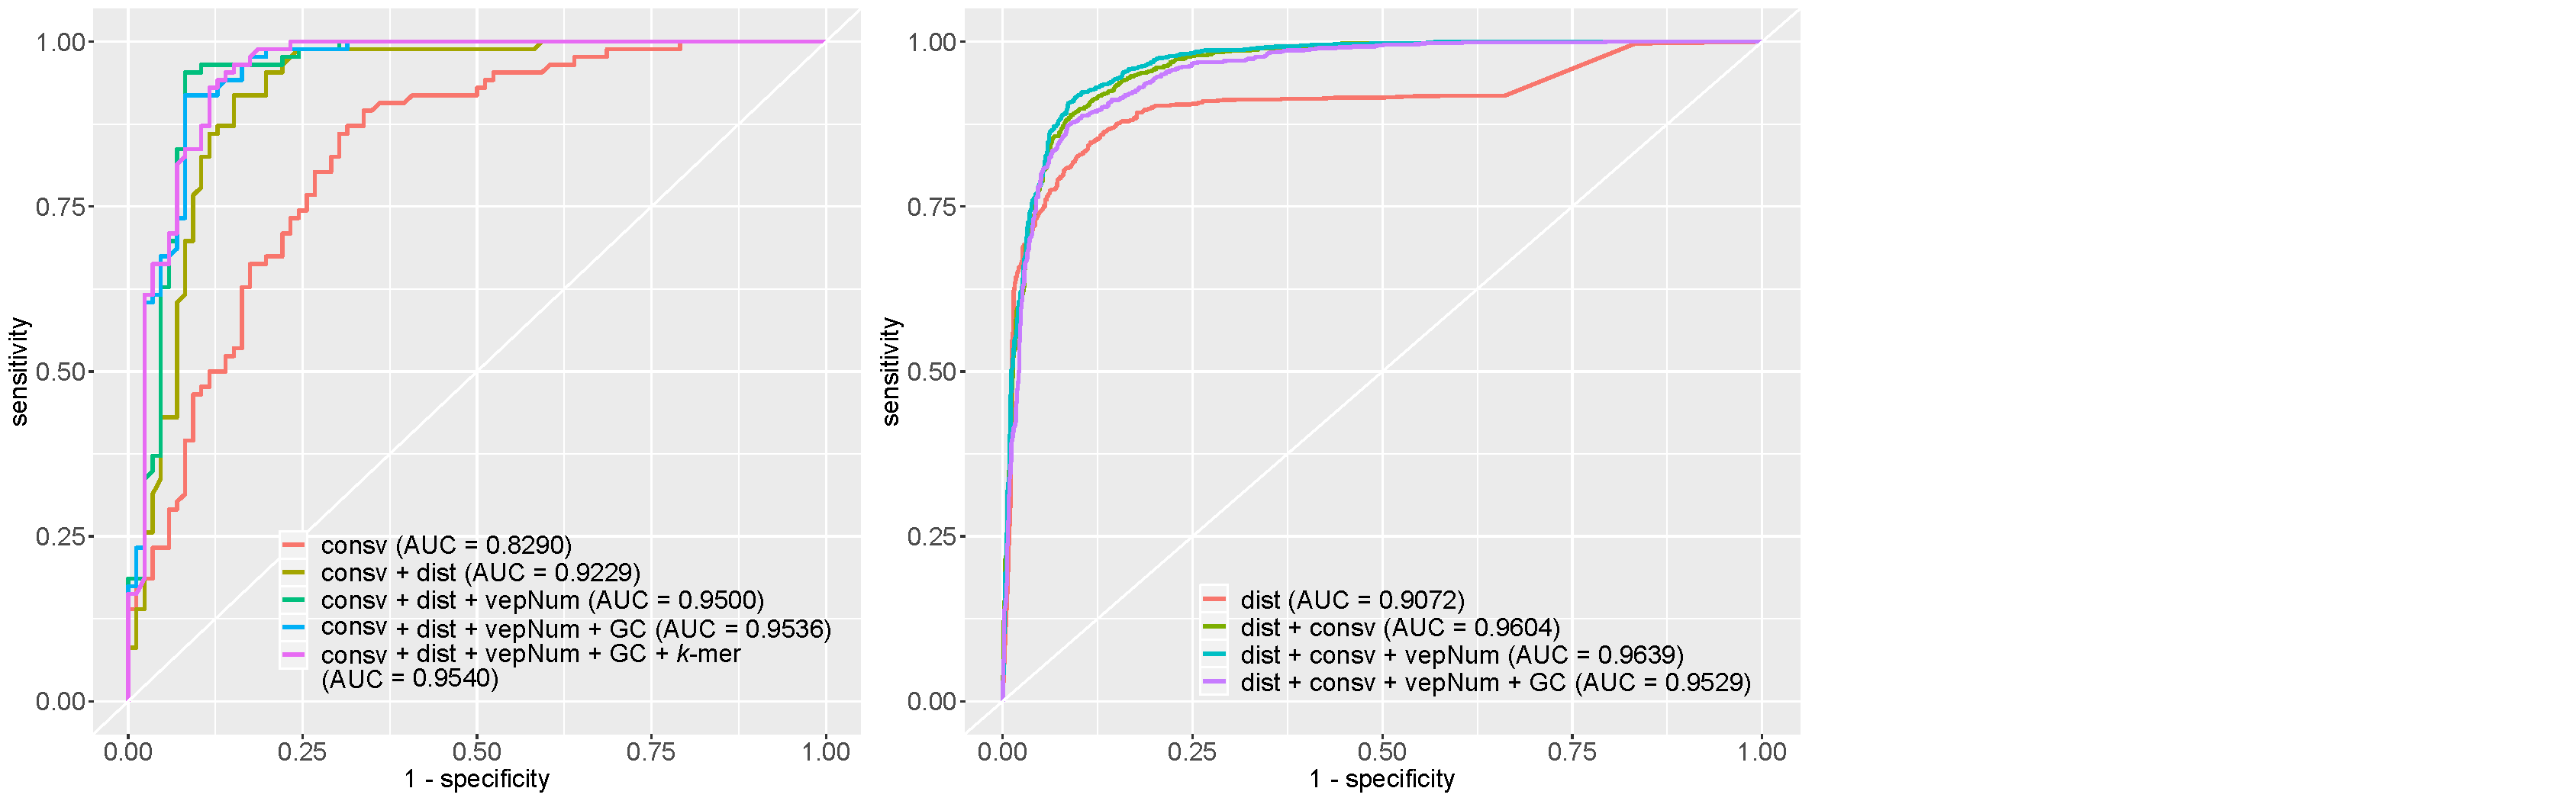
\includegraphics[width=\linewidth]{ROC_FeaComb.pdf}%

  \stepcounter{figure}
  \smallskip\noindent\small Figure \thefigure:
  ROC curves of different feature combinations for coding (left) and non-coding (right) regions.
  %
  \label{fig:ROC_feaComb}%
\end{figure*}

\begin{table}[h!]
  \begin{center}
    \footnotesize%
    \begin{tabular}{p{6.5cm} rrrrr}
      \toprule
      Feature group & Sensitivity & Specificity & Accuracy & F-Measure & Kappa \\
      \midrule
    dist$^1$ + consv$^2$                                & 0.8755 & 0.9154 & 0.8954 & 0.8933 & 0.7909 \\
    dist + vepNum                               & 0.9287 & 0.8137 & 0.8712 & 0.8782 & 0.7424 \\
    dist + GC$^3$                                    & 0.8441 & 0.8945 & 0.8693 & 0.8659 & 0.7386 \\
    dist + \emph{k}mer$^4$                                 & 0.7842 & 0.7757 & 0.7799 & 0.7809 & 0.5599 \\
    dist + vepCons                              & 0.8070 & 0.7300 & 0.7685 & 0.7771 & 0.5371 \\\midrule
    dist + consv + vepNum                       & 0.8802 & 0.9278 & 0.9040 & 0.9017 & 0.8080 \\
    dist + consv + GC                         & 0.8546 & 0.8935 & 0.8740 & 0.8715 & 0.7481 \\
    dist + consv + vepCons                      & 0.7842 & 0.8745 & 0.8294 & 0.8213 & 0.6587 \\
    dist + consv + \emph{k}mer                         & 0.8051 & 0.8213 & 0.8132 & 0.8117 & 0.6264 \\\midrule
    dist + consv + vepNum + GC                  & 0.8593 & 0.9078 & 0.8836 & 0.8807 & 0.7671 \\
    dist + consv + vepNum + vepCons             & 0.7918 & 0.8878 & 0.8398 & 0.8318 & 0.6797 \\
    dist + consv + vepNum + \emph{k}mer                & 0.8156 & 0.8279 & 0.8218 & 0.8207 & 0.6435 \\\midrule
    dist + consv + vepNum + GC + vepCons        & 0.8451 & 0.8916 & 0.8683 & 0.8652 & 0.7367 \\
    dist + consv + vepNum + GC + \emph{k}mer           & 0.8184 & 0.8203 & 0.8194 & 0.8192 & 0.6388 \\\midrule
    dist + consv + vepNum + GC + vepCons + \emph{k}mer & 0.8137 & 0.8232 & 0.8184 & 0.8176 & 0.6369 \\
        % All six feature groups & 0.8137 & 0.8232 & 0.8184 & 0.8176 & 0.6369 \\
      \bottomrule
    \end{tabular}
  \end{center}
  \caption{Performance of different feature combinations for coding regions. Random forest classifier is built using training and validation set, and parameters are fine-tuned using 10-fold CV.\\
  $^1$conservation score; $^2$distance score; $^3$G + C content; $^4$\emph{k}-mer counts.}
  \label{tab:FeaComb_NC}
\end{table}

We further evaluate each feature group using ROC curve (see Figure 7.5). Features for non-coding region generate much smoother curves than features for coding region since the test set of coding region only contains 172 (86 positive and 86 negative) variants. Feature group distance score yield best AUC (Area Under Curve), 0.8519 for coding region and 0.9072 for non-coding region. The second-best feature group is conservation score which produce AUC 0.8290 and 0.7693 for coding and non-coding regions, respectively.

In the following experiments, we hope to find out the optimal feature combinations for coding and non-coding regions. Using sequential learning strategy, the optimal feature combination for non-coding region will be determined in five rounds of evaluation, while coding region needs six rounds.

The results of feature combination are displayed in Table \ref{tab:FeaComb_CD} and Table \ref{tab:FeaComb_NC}. In the first round of evaluation, the combination, conservation score (consv) and distance score (dist), yields the highest accuracy 0.8721 for coding regions and 0.8954 for non-coding regions. Thus, other feature groups are added to this combination in the second round of evaluation.

For coding model, vepNum and feature group G + C content on 9 nt sub-sequence boost the performance of original combination to 0.8895 and 0.8779, respectively. But other feature groups, including vepCons, vepAA and 1-mer counts on 3 nt sub-sequence (\emph{k}-mer features), have deleterious effects on the optimal feature combination of round 1 evaluation. Having combined G + C content with the optimal combination of round 2 evaluation (i.e. conservation score, distance score and vepNum), we find the classifier shows no improvement in accuracy, and the F-measure even drops. In round 4 evaluation, \emph{k}-mer features are incorporated into random forest classifier and improve accuracy from 0.8895 to 0.8953. But feature groups vepCons and vepAA cannot further improve the accuracy. Thus, five feature groups, namely conservation score, distance, vepNum, G + C content and \emph{k}-mer features, are selected to build classifier for coding region.

As to model for non-coding regions, when feature vepNum is added to the optimal feature combination of round 1 (distance and conservation score), the accuracy is increased to 0.9040. In the subsequent evaluations, none of other feature groups can further enhance the performance. It seems that this feature combination can yield satisfactory prediction results, nonetheless, all the features in the optimal combination (distance, conservation and vepNum) are only related to the mutation position in the genome, which makes the model only suitable for biallelic SNVs. Different mutations of the same mutated point may have different impacts on organism. The nucleotide "G" located in position 136,405,929 of the reference genome of X chromosome, for example, can be mutated to "A" or "C". If the mutation is "C", this variant is highly likely to be a pathogenic one, while mutation "A" is relatively neutral. But two different mutations will have the identical features as distance, conservation and vepNum are calculated based on genome position only. To improve model's generalisation, another feature group, G + C content, is also selected to build classifier. The decrease in accuracy (from 0.9040 to 0.8836) is minor when this feature group is added, but the model could give more reliable results for multiallelic variants. For non-coding model, four feature groups, namely conservation score, distance score, vepNum and G + C content, are determined to construct classifier.

ROC curve is also used to evaluate the performance of different feature combinations (see Figure 7.6). For coding model, AUC steadily increases when new feature groups being incorporated into the classifier and reaches 0.9540 for optimal combination. Using our determine feature combination (distance score, conservation score, vepNum and G + C content), non-coding model obtains AUC 0.9529 which is slightly lower than the highest AUC generated by feature combination distance score, conservation and vepNum.

Based on the mean decrease in Gini of random forest classifier, importance score of each feature is calculated using following equation:

\begin{equation}
    \text{Importance Score} = \frac{MeanDecreaseGini - \text{min}(MeanDecreaseGini)}{\text{max}(MeanDecreaseGini) - \text{min}(MeanDecreaseGini)} \nonumber
\end{equation}

Importance scores of features are shown in Table \ref{tab:ImpScore}. Models for coding and non-coding regions share the identical top 5 features: 30-way phyloP and PhastCons scores, distances to start codon, UTR and stop codon. The importance scores of 30-way conservation features are higher than those of 100-way conservation features, which implies oncogenic mutation is more sensitive to multiple alignments between human and mammalian genomes than alignments between human and vertebrate.

\begin{table}[t]
        \begin{center}
        \begin{tabular}{lrclr}
        \toprule
         \multicolumn{2}{c}{Model for coding region} & &\multicolumn{2}{c}{Model for non-coding region}\\
        \cmidrule(l){1-2}
        \cmidrule(l){4-5}
        Feature & Importance Score & \quad & Feature & Importance Score \\
        \midrule
    30-way phyloP         & 100.00 &  & 30-way phylop         & 100.00 \\
    30-way PhastCons      & 83.07  &  & 30-way PhastCons      & 96.02  \\
    distance.start\_codon & 70.41  &  & distance.start\_codon & 83.54  \\
    distance.UTR          & 61.14  &  & distance.UTR          & 83.39  \\
    distance.stop\_codon  & 57.40  &  & distance.stop\_codon  & 54.84  \\
    vepNum                & 52.49  &  & distance.exon         & 54.68  \\
    100-way phyloP        & 37.73  &  & distance.CDS          & 53.93  \\
    ALT\_GC               & 28.74  &  & 100-way phyloP        & 31.22  \\
    100-way PhastCons     & 22.29  &  & REF\_GC               & 25.16  \\
    REF\_GC               & 21.15  &  & distance.transcript   & 18.57  \\
        \bottomrule
        \end{tabular}
        \end{center}
    \caption{Importance score of features for coding and non-coding regions. The scores are computed using the mean decrease in Gini of random forest classifier. Only the top 10 features are listed in the table.}
    \label{tab:ImpScore}
\end{table}

\section{Model Evaluation}

\begin{table}[b!]
  \begin{center}
    \begin{tabular}{lrrrrr}
      \toprule
      Model & Sensitivity & Specificity & Accuracy & F-Measure & Kappa \\
      \midrule
        Logistic regression & 0.6395 & 0.7326 & 0.6860 & 0.6707 & 0.3721 \\
        SVM                 & 0.6860 & 0.8139 & 0.7500 & 0.7329 & 0.5000 \\
        Random forest       & 0.8256 & 0.9651 & 0.8953 & 0.8875 & 0.7907 \\
        GBM                 & 0.8372 & 0.9651 & 0.9012 & 0.8944 & 0.8023 \\
      \bottomrule
    \end{tabular}
  \end{center}
  \caption{Performance of three different machine learning model evaluated on test set for coding regions.}
  \label{tab:perf_mod_CD}
\end{table}

\begin{table}[b!]
  \begin{center}
    \begin{tabular}{lrrrrr}
      \toprule
      Model & Sensitivity & Specificity & Accuracy & F-Measure & Kappa \\
      \midrule
        Logistic regression & 0.6730 & 0.6721 & 0.6725 & 0.6727 & 0.3451\\
        SVM                 & 0.6749 & 0.7519 & 0.7134 & 0.7019 & 0.4268 \\
        Random forest       & 0.8593 & 0.9078 & 0.8836 & 0.8807 & 0.7671 \\
        GBM                 & 0.8935 & 0.9249 & 0.9092 & 0.9078 & 0.8184 \\
      \bottomrule
    \end{tabular}
  \end{center}
  \caption{Performance of three different machine learning model evaluated on test set for non-coding regions.}
  \label{tab:perf_mod_NC}
\end{table}

The machine learning model used by CScape-X is determined with model selection experiments. In addition to random forest, logistic regression, SVM and GBM are also employed to build classifier. Evaluated using 10-fold CV and parameter tuning, the final classifier will be constructed with the algorithm that obtains the highest accuracy. The results are displayed in Table \ref{tab:perf_mod_CD} (models for coding regions) and Table \ref{tab:perf_mod_NC} (models for non-coding regions). ROC curves are also generated to further assess the performance of each tool (see Figure 7.7, left: ROC curves of models for coding regions, right: ROC curves of models for non-coding regions).

We first use logistic regression to build classifiers. For each fold in CV, the cut-off that achieves the highest sensitivity + specificity value will be selected as the optimal cut-off for the classifier. The final cut-off is the average of the optimal cut-offs of all the folds. According to our experiments, the final cut-off for coding region is 0.4613, and for non-coding region is 0.4800. We used these final cut-off values to predict the test sets of coding and non-coding regions. Logistic regression classifier for coding region got accuracy 0.6860, while for non-coding region got 0.6725. The AUC values of the logistic regression models for coding and non-coding regions are 0.7654 and 0.7395, respectively.

Widely-used algorithm SVM is also used to train classifier. Here Radial Basis Function (RBF) is selected as the kernel, and parameters cost (C) and gamma are tuned using 10-fold CV. In this study, C ranges from $2^0$ to $2^5$, and gamma ranges from $2^{-5}$ to $2^1$. Thus, a total of 36 models are evaluated using 10-fold CV. Statistics accuracy is used to determine the optimal parameter combination. For coding regions, the best accuracy 0.7500 occurs at C = $2^3$ and gamma = $2^{-5}$; C = $2^4$ and gamma = $2^{-3}$ yield highest accuracy 0.7134 for non-coding regions. The model trained with SVM is better than that trained with logistic regression and gets AUC 0.8213 and 0.7928 on coding and non-coding region, respectively.

Random forest is selected as default algorithm in this study to evaluate different feature groups. And neither logistic regression nor SVM could outperform random forest who achieves accuracy 0.8953 on coding region and 0.8836 on non-coding region. As an ensemble learning method, random forest produces satisfactory results for this research.

Another decision tree-based ensemble learning method, GBM is also employed to build classifier. Just like the strategy we used to train logistic regression and SVM, we tune GBM and determine the optimal cut-off with 10-fold CV. And the following candidate values are used for parameter tuning: shrinkage (learning rate) = {0.01, 0.05, 0.1}, maximum depth = {3, 5, 7}, minimum number of observations in the terminal nodes (min\_obs) = {5, 7, 10}, subsampling fraction = {0.65, 0.8, 1} and total number of trees = {8,000}. Thus, 81 models determined by different parameter combinations are evaluated using 10-fold CV. Statistics MSE (mean squared error) of CV is used to evaluate different parameter combinations. For coding region, the optimal parameter combination {shrinkage = 0.05, maximum depth = 7, min\_obs = 10, subsampling fraction = 0.65} shows the minimum MSE, 0.6854, when number of tree equals 373. For non-coding region, combination {shrinkage = 0.10, maximum depth = 7, min\_obs = 10, subsampling fraction = 1} shows the minimum MSE, 0.6854, when number of tree = 1468. Afterwards, on the condition that classifiers are trained with optimum parameters, we calculate the best cut-off values (based on 10-fold CV) for coding and non-coding regions. Model for coding region achieves the highest sensitivity + specificity when cut-off equals 0.4884, at which time it yield accuracy 0.9012. For non-coding region, classifier achieves accuracy 0.9092 when best cut-off 0.4230 is selected. In our experiments, GBM outperforms other machine learning methods with highest accuracy and F-measure on both coding and non-coding region. As shown in Figure 7.7, GBM also obtains the highest AUC (0.9689 for coding region and 0.9657 for non-coding region) among four machine learning methods. Thus, GBM is selected to build classifier for CScape-X.

\begin{figure*}[h!]
  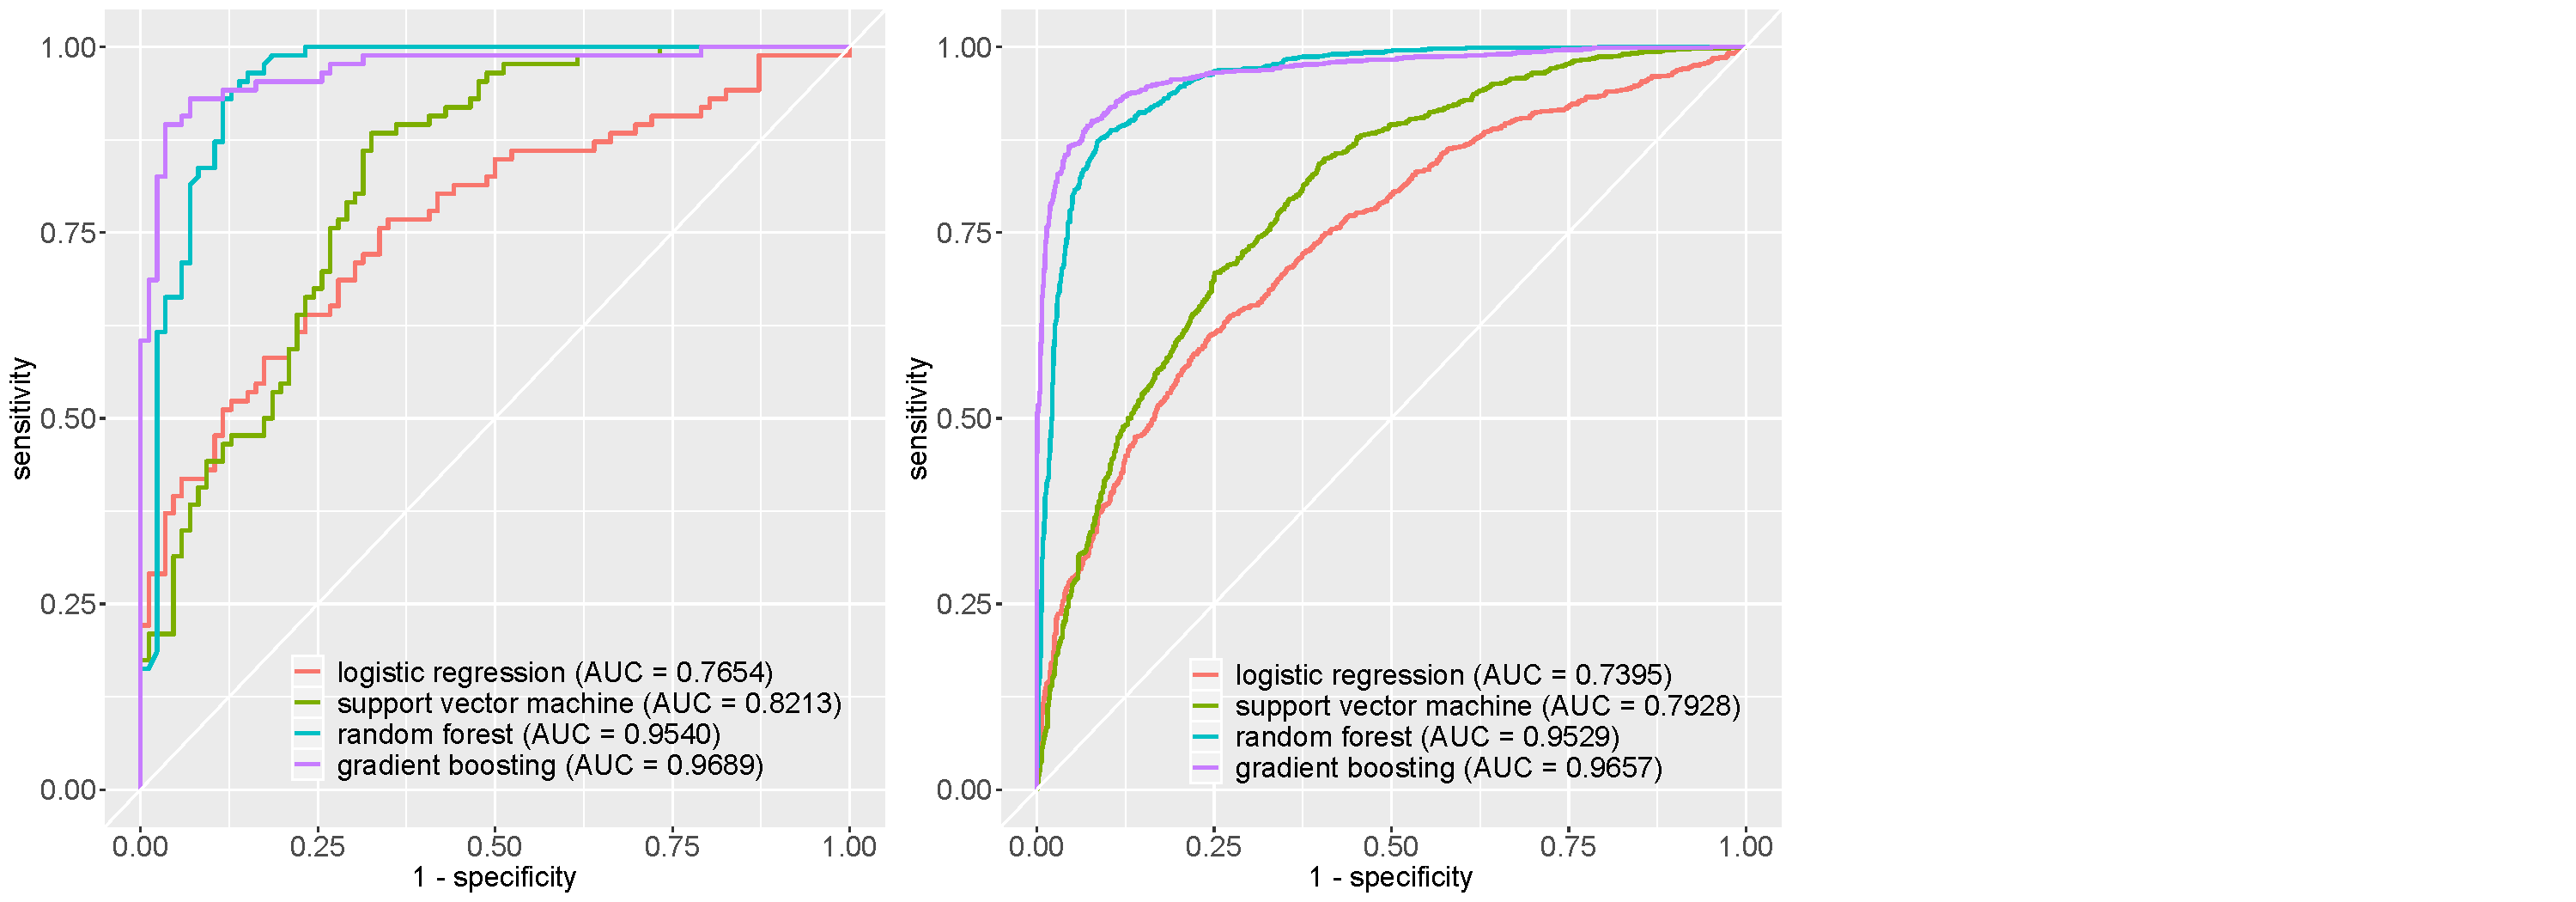
\includegraphics[width=\linewidth]{ROC_multzMod.pdf}

  \stepcounter{figure}
  \smallskip\noindent\small Figure \thefigure:
  ROC curves of different models for coding (left) and non-coding (right) regions. The model are built with four machine learning algorithms, including logistic regression, SVM, random forest and GBM.
  %
  \label{fig:ROC_multzMod}%
\end{figure*}

\section{Comparison with Existing Methods}

\begin{table}[b]
        \begin{center}
        \begin{tabular}{lrrcrr}
        \toprule
         \multirow{2}{*}{Feature group}&\multicolumn{2}{c}{Accuracy (coding region)} & &\multicolumn{2}{c}{Accuracy (non-coding region)}\\
        \cmidrule(r){2-3}
        \cmidrule(r){5-6}
        & CScape-X & CScape & \quad & CScape-X & CScape \\
        \midrule
        conservation score    & \textbf{0.756} & 0.655 & & \textbf{0.862} & 0.572 \\
        VEP (all)             & \textbf{0.723} & 0.674 & & 0.588 & \emph{NA}  \\
        distance score        & \textbf{0.756} & 0.605 & & \textbf{0.862} & 0.515  \\
        G + C content         & 0.634 & \emph{NA} & & 0.650   & \emph{NA} \\
        \emph{k}-mer features & \textbf{0.605} & 0.597 & & \emph{NA} & 0.570   \\
        overall               & \textbf{0.895} & 0.714 & & \textbf{0.909} & 0.586 \\
        \bottomrule
        \end{tabular}
        \end{center}
    \caption{Accuracy of the similar feature groups employed by CScape and CScape-X. The results of CScape are calculated from LOO-CV and collected from its original paper. And the results of CScape-X is calculated from 10-fold CV. Bold numbers indicate the higher values.}
    \label{tab:compare}
\end{table}

In this section, we try to benchmark CScape-X against existing tools. However, it is not easy to compare CScape-X with other methods. Some tools, such as FATHMM-MKL and GWAVA \cite{Ritchie2014}, only support version GRCh37 of human genome, but CScape-X is built with updated GRCh38 version which is quite distinct from GRCh37. Some state-of-the-art tools, such as CScape and FATHMM-XF, support GRCh38, but cannot be applied to X chromosome. Due to the time constraint, it is impossible to re-implement and retrain existing tools with the same training sets used by CScape-X, here we can only adopt some strategies to compare their performance indirectly.

CScape, the precursor of CScape-X, is first used to benchmark CScape-X. The performance of CScape is collected from original paper \cite{Rogers2017}. Seems that it is neither sensible nor informative to compare two sets of statistics that come from different datasets. But CScape-X is similar to its predecessor from the perspective of feature design. By comparing the performance of CScape-X's feature groups with those of corresponding feature groups of CScape, we can roughly estimate if CScape-X performs better than CScape on X chromosome. The results are summarised in Table \ref{tab:compare}. The accuracies of CScape-X are computed from 10-fold CV, and the results of CScape are from leave-one-chromosome-out cross validation (LOCO-CV). Table \ref{tab:compare} demonstrates the performance of CScape-X on X chromosome is better than that of CScape on autosomes. We can also notice that \emph{k}-mer features display similar performance on autosomes and X chromosome, but conservation score, VEP-based features and distance scores show better results on X chromosome. These three features are directly or indirectly based on genome annotation. CScape-X uses the latest annotation information, which may boost classifier's performance and help CScape-X achieve higher accuracy.

To have a comprehensive evaluation, CScape-X is also benchmarked against method CADD. CScape-X and CADD are evaluated using the identical test set. Since CADD provides no threshold for its prediction, ROC curves (see Figure 7.8) are used to evaluate CADD and CScape-X. For variants in coding region, CScape-X achieves AUC 0.9689, while CADD got 0.6322. CScape-X also outperforms CADD (AUC = 0.5923) on non-coding region with AUC 0.9657.

In this section, CScape-X is briefly compared with CScape and CADD. Although it is not a fair comparison since CScape-X and its competitors have not been trained with the same training set, it is still clear that CScape-X can give satisfactory results for oncogenic SNV prediction.

\begin{figure*}[t!]
\centering
  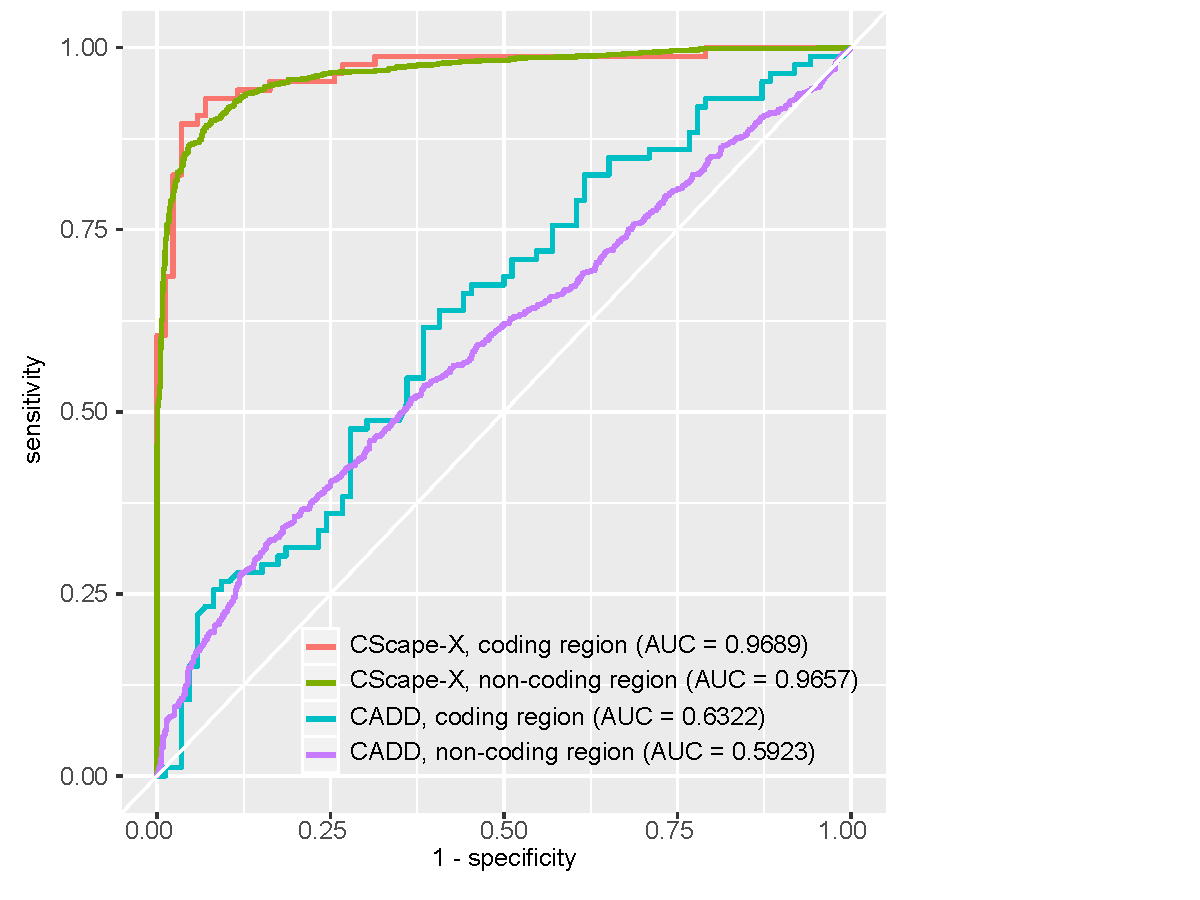
\includegraphics[width=0.75\linewidth]{ROC_CADD.pdf}%

  \stepcounter{figure}
  \smallskip\noindent\small Figure \thefigure:
  ROC curves of CScape-X and CADD evaluated on coding and non-coding region.
  \label{fig:CADD}%
\end{figure*}

% \clearpage
\section{Analysis of Computational Speed}

\begin{figure*}[t]
  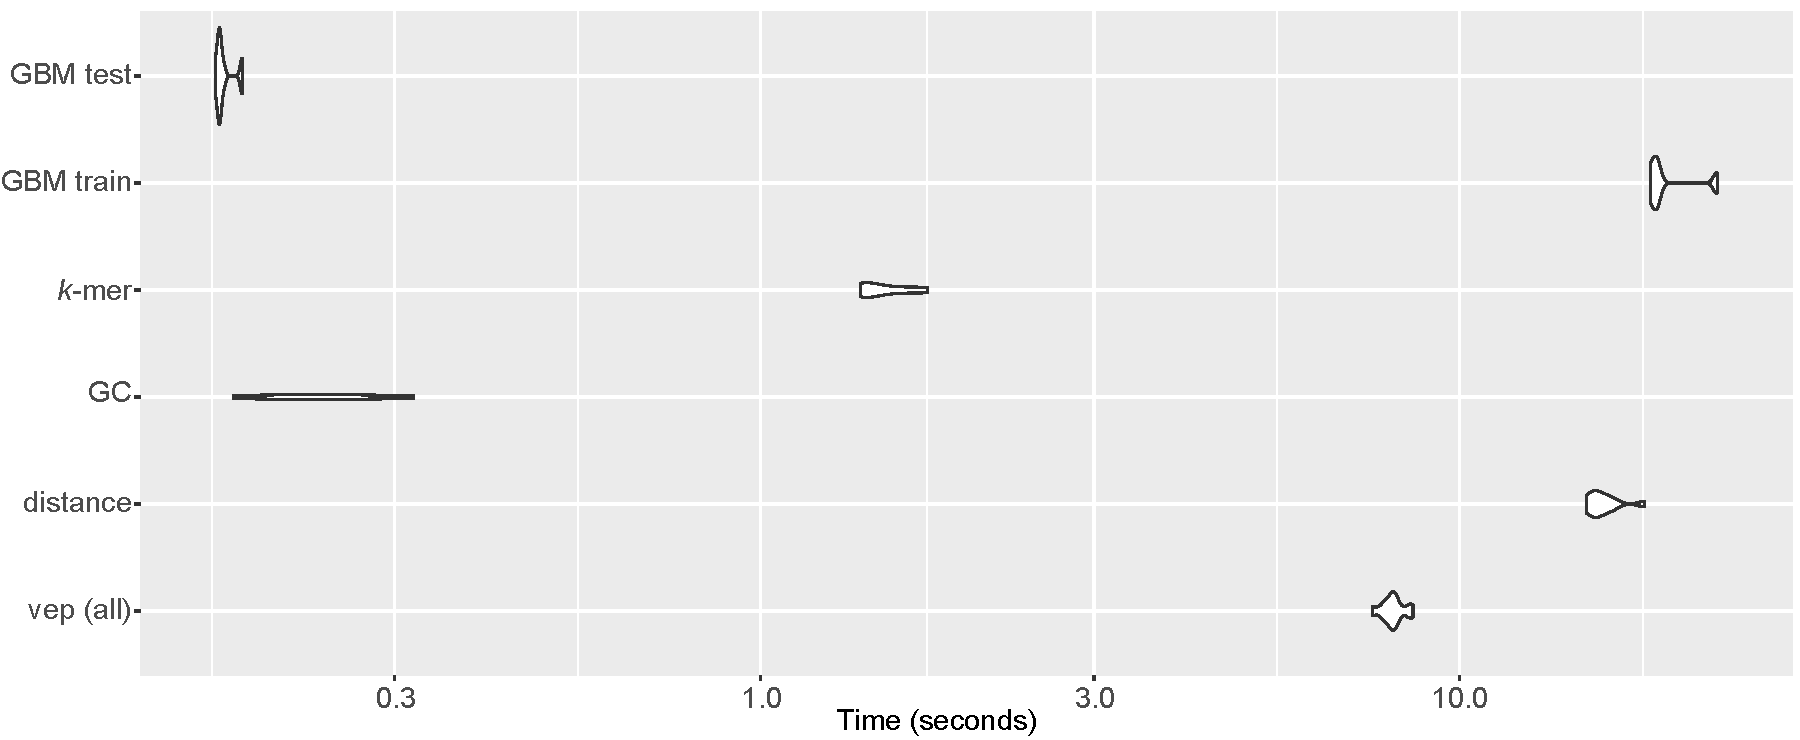
\includegraphics[\linewidth]{timeEval.pdf}%

  \stepcounter{figure}
  \smallskip\noindent\small Figure \thefigure:
  Time speed analysis of feature extraction and classifier construction. This results in this violin plot is based on the experiments that all expressions are evaluated 10 times. The training set for GBM construction contains 8,416 variants, while the dataset for feature extraction and prediction contain 4,000 variants. GBM classifier in this evaluation is trained using 10-fold CV with parallel computing on 10 cores, but no paramer tuning is performed. The running time of feature extraction is measured with one core. \emph{k}-mer features are extracted from 3 nt sub-sequences with \emph{k} = 1; G + C content is computed on 9 nt sub-sequences; the width of distance-derived feature is set as 85,000; VEP-based feature groups include features from three subgroups (vepNum, vepCons and vepAA), though only one of them (vepNum) is finally selected to build CScape-X.
  \label{fig:time_eval}%
\end{figure*}

The computational speed of CScape-X is finally analysed. We use the same platform to measure the running time of feature extraction and classifier construction. Each command will be evaluated 10 times. Since conservation scores are provided by UCSC genome browser, we here only analyse other types of feature groups. The platform configurations for this evaluation are 32 Intel$\textregistered$ Xeon$\textregistered$ E5-2640 processors @ 2.60 GHz, 256 GB memory and 64 bits Linux OS. The results are displayed in Figure 7.9.

It only takes around 0.239 seconds to extract G + C content features from 4,000 variants, while 16.08 seconds are required to calculate distance-derived features. Our scripts use 8.040 seconds to extract all three kinds of features (vepNum, vepCons and vepAA) of VEP group. Only feature vepNum is selected for classfier construction, and it only takes 0.046 seconds to extract this feature. As to \emph{k}-mer features, it takes 1.506 seconds to extract 1-mer counts on 3 nt sub-sequences. In our evaluation, 10-fold CV is used to train GBM and determine the optimum cut-off. With parallel computing (10 cores), it takes about 19.871 seconds to complete the process. Using GBM classifier, CScape-X can predict 4,000 variant in just 0.171 seconds.

The total time cost of determining optimal window width, including parameter tuning with 10-fold CV, for distance-based and \emph{k}-mer features is about 5 days with parallel computing (10 cores). The time cost of the evaluation of different feature combinations is about 2 days with parallel computing on 10 cores.

The experimental results have proved that CScape-X can predict oncogenic SNVs effectively and efficiently. In subsequent work of this project, CScape-X will be published as a database supporting online/offline retrieval, which could provide instant access to all pre-computed results.

\clearpage
\chapter{Critical Evaluation}

In spite of limited time, we aim to present a reliable method for oncogenic SNV prediction and make the research as comprehensive as possible. Nevertheless, there still remain some issues and challenges. In this chapter, we will discuss our method from two aspects: 1) design and development and 2) evaluation and results. We hope the evaluation of this part can bolster the subsequent work of this research.

\section{Design and Development}

During the data collection, the neutral variants were firstly collected from a comprehensive release of 1000 Genomes Project. However, the neutral variants cannot match the positive variants collected from COSMIC. A latest version is then downloaded from 1000 Genomes Project. Data from this version can match COSMIC, but it only contains limited variants from non-coding region. Compared with dataset for non-coding region which consists 10,520 variants, dataset for coding region only contains 864 variants. Insufficient data could easily affect subsequent feature evaluation and weaken the generalisation of final classifier.

To economise on time, we used recurrence threshold proposed by CScape to construct high-standard datasets for CScape-X. However, this threshold is experimentally verified on autosomes, and the proper threshold for X chromosome may be different.

In this project, seven kinds of features, namely conservation scores, vepNum vepCons, vepAA, distance score, \emph{k}-mer counts and G + C content, are extracted to build the classifier. Now we will take a look at each of these feature.

\textbf{Conservation scores (PhastCons and phyloP)} yield the best accuracy on coding as well as non-coding regions. Considering that 30- and 100-way conservation scores show satisfactory results in our study, it is also worth exploring other types of scores, such as 7- or 20-way scores. One limitation of conservation scores (as well as distance-derived features and feature vepNum) is that, these features are irrelevant to mutated nucleotides---they are only based on positions in the genome. To make conservation-based features capture the affects caused by different mutations at the same position, substitution rate of different nucleotides can be computed using multiple alignments. However, it will be an extremely arduous task to align the whole chromosome against the genomes of other species.

\textbf{VEP-based feature group}, including vepNum, vepCons and vepAA three kinds of features, is designed based on the results provided by VEP which can measure the effect of the variants on gene sequences. In original CScape paper, VEP-based features are regarded as one kind of features and only used to build the classifier for coding region, since vepAA features are inapplicable to variants from non-coding region. In this study, vepNum, vepCons and vepAA are regarded as three kinds of features. Although vepAA features are irrelevant to non-coding region, vepNum and vepCons can contribute towards classifier for non-coding region. Based on the results of different feature combinations, vepNum feature enhances the performances of the classifiers for both coding and non-coding region. Apart from vepNum, vepCons, and vepAA, many other useful pieces of information such as pathogenicity predictions of other tools and impact level of the mutation (high, moderate, modifier, low) can also obtained using VEP. However, we did not include these data into our feature set in order to mitigate potential bias.

\textbf{Distance scores}, in this study, are calculated by measuring the distance from mutated point to several gene features, including gene, transcripts, UTR, CDS, start codon, stop codon and exon. But we notice that, almost all SNVs are located in transcripts and genes, and almost all the variants from coding region are located in CDS. Thus, the contribution of distances between SNVs and these gene features is extremely limited, even negligible. Due to the insufficient time, we here use all distance scores to train classifier, but a feature selection process can be performed using all variants collected from X chromosome to test whether some distance scores can be eliminated to streamline the feature set. Additionally, if all SNVs are located in genes (so the distance score = 1), can we further extract features by measuring the positions of SNVs in genes? Many motifs, such as the core sequences of enhancer, play important role in transcription and translation, can we extract features by scanning if mutations are located in some critical motifs? Apart from distance score, many useful features could be designed using genome annotation.

\textbf{\emph{k}-mer features} show the alteration of the genomic context caused by the variants. Unlike CScape who uses \emph{k}-mer counts only, two strategies, \emph{k}-mer counts and \emph{k}-mer frequencies, are tested in this study to build CScape-X. Several combinations of window width and \emph{k} value are evaluated as well. Width 3 nt and \emph{k} 2 are used by CScape to build model for both coding and non-coding region of autosomes. In our test, width = 3 nt and \emph{k} = 1 generated best result for coding region of X chromosome, while width = 9 nt and \emph{k} = 3 showed highest accuracy for non-coding region of X chromosome. We also found that the matrices of \emph{k}-mer counts are very sparse. Too many zeros in \emph{k}-mer count will introduce noise and affect the performance of the classifier. To reduce the potential noise, some strategies may be applied to refine \emph{k}-mer features. In my previous research \cite{Han2018}, I designed Logarithm-Distance and Euclidean-Distance to reduce the dimension of \emph{k}-mer features. Although I hardly have time to validate the performance of these two schemes on this topic, independent reseach \cite{Amin2019} demonstrated that these two distance scores can capture the alterations in \emph{k}-mer features on a macro-level, which means they may benefit oncogenic SNV prediction as well.

\textbf{G + C content} is also evaluated on sub-sequences of different lengths (from 1 to 9 nt). Although CScape does not select G + C content to train classifier, this feature show satisfactory result in our evaluation. The accuracy of G + C content improves with the increase of sub-sequence length. More different widths of the sub-sequence can be tested to achieve the best results.

As to classifier construction, four machine learning methods, namely logistic regression, random forest, SVM and GBM, are evaluated with parameter tuning. Perhaps the features designed in this study cannot perfectly characterise oncogenic SNVs. Classifier with the strongest learning ability achieves the highest accuracy. Deep learning methods also have very high learning ability. However, tuning deep learning model is time-consuming, and the limited variants from coding region can easily cause over-fitting of complicated models. To avoid over-fitting, 10-fold CV is used to test the models trained with different methods. Regularisation techniques may also be used to enhance model's generalisation ability.

This project mainly focuses on the design of CScpae-X. But for the next stage, CScape-X is expected to release as a web server. The development and release of CScape-X pacakge and web server will be briefly discussed in section Future Work.

\section{Evaluation and Results}

For variants in coding region, conservation scores and distance scores achieved the highest accuracy 0.7558. Although feature vepNum only got an accuracy of 0.5581, it can further improve classifier's performance. The combination of these three feature groups can yield accuracy 0.8895. After adding \emph{k}-mer features and G + C content, the accuracy climbed to 0.8953. When we use GBM to build classifier, this feature combination achieves accuracy 0.9012 and F-measure 0.8944.

For variants in non-coding region, distance scores still wield the greatest discriminating power. Combined with conservation scores and vepNum, model for non-coding region can achieve accuracy 0.9040. But all these features are only related to allele positions, regardless of mutated allele nucleotides. Feature G + C content is also included into feature set so that the classifier can capture the affects caused by multiallelic variants. The final GBM model obtained accuracy 0.9092 and F-measure 0.9078 on non-coding region.

Compared with CScape and CADD, CScape-X displays satisfactory results for the prediction of oncogenic SNV from X chromosome. Several reasons may account for this result:
\begin{itemize}
  \item The improvement in genome annotation has also improved the quality of features, which further boosted the performance of classifier.
  \item CScape and CADD are trained with features extracted from autosomes or the whole genome, while CScape-X is tailored for X chromosome. Data used by CScape-X are relatively homogeneous, and the classifier can better grasp the underlying patterns.
  \item Also, it should be noted that the datasets, especially the datasets for coding region, used in study are not comprehensive enough. The prediction could be unduly optimistic if the datasets fail to properly portray the whole X chromosome.
\end{itemize}

To make CScape-X a reliable and robust tool, further exploration and validation with large datasets are necessary. Genome assembly GRCh37 may also be used to validate CScape-X.

\clearpage
\chapter{Summary}

In this study, a novel method, CScape-X, is proposed to facilitate the research on oncogenic SNV prediction. Currently, the design and development of CScape-X method are basically completed. However, there is still some work to be done before the release of CScape-X.

\section{Future Work}

Based on our critical evaluation, several limitations of this study can be addressed in subsequent work. For example, large and comprehensive datasets can be constructed using GRCh37 as well as GRCh38 assembly. Optimum recurrence threshold for X chromosome need to be determined. For feature engineering part, other kinds of conservation scores, such as 7-Way and 20-Way PhastCons and phyloP scores, can be evaluated; a more sophisticated tuning on distance score and \emph{k}-mer features can be carried out.

Moreover, more innovative features, for example the alteration in binding hotspots, can be incorporated into the classifier. A hot spot is a site on a target protein that has high propensity for ligand binding \cite{Zerbe2012}. Studies show that proteins can selectively bind to other molecules and perform specific functions \cite{Chen2016}. Thus, if one variant is located in these binding hotspots, substitution of amino acids could alter binding hotspot and further cause functional affects on organisms. This feature group may contribute to the classifier for coding region. Non-coding sequences are far more than coding sequences in human genome. Low expression level and high tissue specificity of non-coding region make it difficult to characterise SNVs in non-coding region. Even worse, many powerful features are not applicable to non-coding region. Thus, more critical features need to be designed for non-coding region.

CScape-X will be finally released as web server. Users can obtain predicted results by uploading a .vcf file or entering mutation position, mutated nucleotide and reference nucleotide (original allele base in the reference genome). During the experiments, we noticed that it is importance to ensure data from difference sources are used the same genome assembly. Thus, not only should the consistency of different data used by CScape-X be checked, but also the consistency between the data provided by users and the data used for CScape-X development should also be examined. If the reference bases provided by users cannot match the reference bases recorded in CScape-X, the results calculated by CScape-X may not match users' data either. To maximise CScape-X's availability and deal with the problem that the genome assembly uploaded by users differ from that used for model construction, CScape-X could also be published as an R package, which can be used to build new models with users' own data.

\section{Conclusion}

This research completes a comprehensive process of the development of bioinformatics tools. Seven types of features from three categories, namely conservation scores, VEP information and genomic context, were extracted and evaluated using 10-fold CV. A comprehensive feature selection process was also conducted to determine the optimum feature combinations for coding and non-coding regions. Moreover, four classifier random forest, logistic regression, SVM and GBM classifier were used to perform model selection to determine appropriate models for CScape-X. A computational speed analysis was finally carried out to show the efficiency of CScape-X.

Currently, about 8.6 billion SNV have been discovered in human genome (more than three million SNVs are located in X chromosome). The high discriminating power of CScape-X can help the tool identify the most compelling variants and provide an effective way to rank predictions for subsequent analysis. Based on reliable performance of CScape-X and comprehensive process of feature selection, we expect CScape-X could guide wet-lab experiments of pathogenic SNV analysis and facilitate a deeper understanding of the role of different features in pathogenic SNV prediction.

\clearpage
\chapter{Availability}

Datasets, scripts and raw results can be download from
\url{https://github.com/HAN-Siyu/UoB_CScape-X}.
\backmatter

\printbibliography
\end{fullwidth}
\printindex

\end{document}
